\chapter{Conceptos básicos}
\label{chap:conceptos basicos}

\section{Generalidad}

Definiremos un grafo como un sistema matemático abstracto. No obstante, para desarrollar el conocimiento de los mismos de forma intuitiva los representaremos mediante diagramas. A estos diagramas les daremos también el nombre de grafos, aun cuando los términos y definiciones no estén limitados únicamente a los grafos que pueden representarse mediante diagramas.

Un grafo es un conjunto de puntos y un conjunto de líneas donde cada línea une un punto con otro. 

\section{Definición formal}

\begin{fondo}
Llamaremos grafo, G, al par ordenado formado por un conjunto finito no vacío, V, y un conjunto, A, de pares no ordenados de elementos del mismo.\\
\smallskip
\quad V es el conjunto de los vértices o nodos del grafo.\\
\smallskip
\quad A será el conjunto de las aristas o arcos del grafo.\\
\smallskip
Utilizaremos la notación G = (V,A) para designar al grafo cuyos conjuntos de vértices y aristas son, respectivamente, V y A.
\end{fondo}

A cualquier arista de un grafo se le puede asociar una pareja de vértices del mismo. Si $u$ y $v$ son dos vértices de un grafo y la arista $a$ esta asociada con este par, escribiremos $a = uv$.\\

Por ejemplo, si\\
\[ V = \{v_1, v_2, v_3, v_4, v_5\} \]
y\\
\[ A = \{v_1v_2, v_1v_3, v_1v_4, v_2v_4, v_2v_5\} \]
entonces el grafo $G = (V,A)$ tiene a $v_1, v_2, v_3, v_4$ y $v_5$ como vértices y sus aristas son $v_1v_2, v_1v_3, v_1v_4, v_2v_4$ y $v_2v_5$.

\section{Tipos de grafos}

\subsection{Grafos lineales}

\begin{fondo}
Sea un grafo $L_n\ $, diremos que es un grafo lineal con $n$ vértices ($n \geq 2$) si tiene $n$ vértices (dos de grado 1 y el resto, si los hay, son de grado 2) y es isomorfo a:
\end{fondo}

\figuratikz{1}{Grafo lineal.}
{
  \tikzstyle{place}=[circle,thick,draw=blue!20,fill=green!20,minimum size=6mm]

  \begin{scope}

    \node [place] (c1)                   {};

    \node [place] (c2) [right of=c1] {}
    edge []                            (c1);

    \node [place] (c3) [right of=c2] {}
    edge [] (c2);

    \node [place] (c4) [right of=c3] {}
    edge []                            (c3);

    \node [place] (c5) [right of=c4] {}
    edge []                            (c4);

    \node [place] (c6) [right of=c5] {}
    edge []                            (c5);

    \node [place] (c7) [right of=c6] {}
    edge []                            (c6);

  \end{scope}  
}

\subsection{Grafos circulares}

\begin{fondo}
Sea un grafo $C_n\ $, diremos que es un grafo circular con $n$ vértices (todos de grado 2), si es $|n| \geq 3$:
\end{fondo}

\figuratikz{1}{Grafo circular.}
{
  \tikzstyle{place}=[circle,thick,draw=blue!20,fill=green!20,minimum size=6mm]
  \tikzstyle{texto}=[]

  \begin{scope}

    \node [place] (c1)                   {};

    \node [place] (c2) [right of=c1,yshift=1.5cm] {}
    edge []                            (c1);

    \node [place] (c3) [right of=c2,yshift=-1.5cm] {}
    edge [] (c2) 
    edge [] (c1);

    \node [texto] (t1) [below of=c2,yshift=-1.4cm,label=above:\textcolor{black}{$C_3$}] {};

    \node[place] (c4) [right of=c3] {};

    \node[place] (c5) [above of=c4,yshift=.5cm] {}
    edge [] (c4);

    \node[place] (c6) [right of=c5,xshift=.7cm] {}
    edge [] (c5);

    \node[place] (c7) [right of=c4,xshift=.7cm] {}
    edge [] (c4)
    edge [] (c6);

    \node[texto] (t2) [below of=c4,label=above:\textcolor{black}{$C_4$},yshift=.1cm,xshift=.9cm] {};

    \node[place] (c8) [right of=c6,xshift=.3cm] {};

    \node[place] (c11) [right of=c7,xshift=1cm] {}
    edge [] (c8);

    \node[place] (c9) [above of=c11,xshift=.65cm,yshift=1.2cm] {}
    edge [] (c8);

    \node[place] (c12) [right of=c11,xshift=.4cm] {}
    edge [] (c11);

    \node[place] (c10) [above of=c12,yshift=.5cm,xshift=.6cm] {}
    edge [] (c12)
    edge [] (c9);

    \node[texto] (t3) [below of=c11,yshift=.1cm,xshift=.8cm,label=above:\textcolor{black}{$C_5$}] {};
\end{scope}
}

\underline{Algoritmo de comprobación: Grafo Circular}\\
\begin{Verbatim}[commandchars=\\\{\}]
\PY{c+cm}{/**}
\PY{c+cm}{ * Método observador.}
\PY{c+cm}{ * Comprueba si el grafo (o componente) es circular o no.}
\PY{c+cm}{ * @return boolean: devolverá true o false si el grafo es o no circular.}
\PY{c+cm}{ * @exception Exception}
\PY{c+cm}{ */}

\PY{k+kd}{public} \PY{k+kt}{boolean} \PY{n+nf}{es\PYZus{}circular}\PY{o}{(}\PY{o}{)} \PY{k+kd}{throws} \PY{n}{Exception}
\PY{o}{\PYZob{}}
    \PY{k+kt}{int} \PY{n}{grado\PYZus{}grafo}\PY{o}{=}\PY{l+m+mi}{0}\PY{o}{;}
    \PY{k+kt}{int} \PY{n}{tama\PYZus{}G} \PY{o}{=} \PY{k}{this}\PY{o}{.}\PY{n+na}{devolver\PYZus{}matriz}\PY{o}{(}\PY{o}{)}\PY{o}{.}\PY{n+na}{length}\PY{o}{;}

    \PY{k}{if}\PY{o}{(}\PY{k}{this}\PY{o}{.}\PY{n+na}{n\PYZus{}nodos}\PY{o}{(}\PY{o}{)} \PY{o}{>}\PY{o}{=} \PY{l+m+mi}{3}\PY{o}{)}
	\PY{o}{\PYZob{}}
	    \PY{k}{for}\PY{o}{(}\PY{k+kt}{int} \PY{n}{i}\PY{o}{=}\PY{l+m+mi}{0}\PY{o}{;} \PY{n}{i} \PY{o}{<} \PY{n}{tama\PYZus{}G}\PY{o}{;} \PY{o}{+}\PY{o}{+}\PY{n}{i}\PY{o}{)}
		\PY{k}{if}\PY{o}{(}\PY{n}{grado\PYZus{}nodo}\PY{o}{(}\PY{n}{i}\PY{o}{,}\PY{k}{this}\PY{o}{.}\PY{n+na}{devolver\PYZus{}matriz}\PY{o}{(}\PY{o}{)}\PY{o}{)} \PY{o}{=}\PY{o}{=} \PY{l+m+mi}{2}\PY{o}{)}
		    \PY{n}{grado\PYZus{}grafo}\PY{o}{+}\PY{o}{+}\PY{o}{;}
		

	    \PY{k}{if}\PY{o}{(}\PY{n}{grado\PYZus{}grafo} \PY{o}{=}\PY{o}{=} \PY{n}{tama\PYZus{}G}\PY{o}{)}
		\PY{o}{\PYZob{}}
		    \PY{n}{System}\PY{o}{.}\PY{n+na}{out}\PY{o}{.}\PY{n+na}{println}\PY{o}{(}\PY{l+s}{"El grafo es circular"}\PY{o}{)}\PY{o}{;}
		    \PY{k}{return} \PY{k+kc}{true}\PY{o}{;}
		\PY{o}{\PYZcb{}}
	\PY{o}{\PYZcb{}}
	
    \PY{k}{return} \PY{k+kc}{false}\PY{o}{;}

    
\PY{o}{\PYZcb{}}
\end{Verbatim}



\subsection{Grafos completos}

\begin{fondo}
Se dice que un grafo es completo cuando todos sus vértices son adyacentes a todos los vértices del grafo, es decir, cuando cada par de vértices son los extremos de una arista. Notaremos por $K_n$ los grafos completos de $n$ vértices.
\end{fondo}

\figuratikz{1}{Grafo completo.}
{
  \tikzstyle{place}=[circle,thick,draw=blue!20,fill=green!20,minimum size=6mm]
  \tikzstyle{texto}=[]

  \begin{scope}

    \node [place] (c1) [label=below:\textcolor{black}{$K_1$}] {};

    \node [place] (c2) [right of=c1, xshift=.2cm, label=below:\textcolor{black}{$K_2$}] {};

    \node [place] (c3) [above of=c2, yshift=.5cm] {}
    edge [] (c2);

    \node [place] (c4) [right of=c2,xshift=.3cm] {};

    \node [place] (c5) [right of=c4,xshift=.5cm] {}
    edge [] (c4);

    \node [place] (c6) [below of=c4,xshift=.8cm,yshift=3.1cm] {}
    edge [] (c4)
    edge [] (c5);

\node [texto] (t1) [below of=c4,xshift=.8cm,yshift=1.1cm,label=below:\textcolor{black}{$K_3$}] {};

    \node [place] (c7) [right of=c5,xshift=.5cm] {};

    \node [place] (c8) [above of=c7,yshift=.5cm] {}
    edge [] (c7);

    \node [place] (c9) [right of=c8,xshift=.5cm] {}
    edge [] (c8)
    edge [] (c7);

    \node [place] (c10) [right of=c7,xshift=.5cm] {}
    edge [] (c9)
    edge [] (c7)
    edge [] (c8);

    \node [texto] (t2) [right of=c7,xshift=-.2cm,label=below:\textcolor{black}{$K_4$}] {};


    \node [place] (c11) [right of=c10,xshift=.3cm] {};

    \node [place] (c12) [right of=c11,xshift=.5cm] {}
    edge [] (c11);

    \node [place] (c13) [below of=c11,xshift=.7cm,yshift=3cm] {}
    edge [] (c11)
    edge [] (c12);

    \node [place] (c14) [above of=c11,xshift=-.4cm] {}
    edge [] (c11)
    edge [] (c12)
    edge [] (c13);

    \node [place] (c15) [above of=c12,xshift=.4cm] {}
    edge [] (c11)
    edge [] (c12)
    edge [] (c13)
    edge [] (c14);

    \node [texto] (t3) [below of=c11,xshift=.8cm,yshift=1.1cm,label=below:\textcolor{black}{$K_5$}] {};

  \end{scope}

}

\underline{Algoritmo de comprobación: Grafo Completo}\\
\begin{Verbatim}[commandchars=\\\{\}]
\PY{c+cm}{/**}
\PY{c+cm}{ * Método observador.}
\PY{c+cm}{ * Comprueba si el grafo (o componente) es completo o no.}
\PY{c+cm}{ * @return boolean: devolverá true o false si el grafo es o no completo.}
\PY{c+cm}{ * @exception Exception}
\PY{c+cm}{ */}

\PY{k+kd}{public} \PY{k+kt}{boolean} \PY{n+nf}{es\PYZus{}completo}\PY{o}{(}\PY{o}{)} \PY{k+kd}{throws} \PY{n}{Exception}
\PY{o}{\PYZob{}}
    \PY{k}{return} \PY{n}{e}\PY{o}{.}\PY{n+na}{es\PYZus{}completo}\PY{o}{(}\PY{o}{)}\PY{o}{;}
\PY{o}{\PYZcb{}}
\end{Verbatim}



\subsection{Grafos vacíos}

\begin{fondo}
Si un grafo tiene $n$ vértices y ninguna arista, estamos ante un grafo vacío.
\end{fondo}

\underline{Algoritmo de comprobación: Grafo Vacío}\\
\begin{Verbatim}[commandchars=\\\{\}]
\PY{c+cm}{/**}
\PY{c+cm}{ * Método observador.}
\PY{c+cm}{ * Comprueba si el grafo (o componente) es vacío o no.}
\PY{c+cm}{ * Esta función comprueba que hay vértice pero no tiene aristas.}
\PY{c+cm}{ * @return boolean: devolverá true o false si el grafo es o no vacío.}
\PY{c+cm}{ * @exception Exception}
\PY{c+cm}{ */}

\PY{k+kd}{public} \PY{k+kt}{boolean} \PY{n+nf}{es\PYZus{}vacio}\PY{o}{(}\PY{o}{)} \PY{k+kd}{throws} \PY{n}{Exception}
\PY{o}{\PYZob{}}
    \PY{k}{if}\PY{o}{(}\PY{k}{this}\PY{o}{.}\PY{n+na}{n\PYZus{}aristas}\PY{o}{(}\PY{o}{)} \PY{o}{=}\PY{o}{=} \PY{l+m+mi}{0}\PY{o}{)}
	\PY{o}{\PYZob{}}
	    \PY{n}{System}\PY{o}{.}\PY{n+na}{out}\PY{o}{.}\PY{n+na}{println}\PY{o}{(}\PY{l+s}{"El grafo es vacío"}\PY{o}{)}\PY{o}{;}
	    \PY{k}{return} \PY{k+kc}{true}\PY{o}{;}
	\PY{o}{\PYZcb{}}
    \PY{k}{else}
	\PY{k}{return} \PY{k+kc}{false}\PY{o}{;}
\PY{o}{\PYZcb{}}
\end{Verbatim}



\subsection{Grafo regular}

\begin{fondo}
Un grafo se dice que es regular cuando todos sus vértices tienen el mismo grado.
\end{fondo}

\subsection{Grafo complementario}

\begin{fondo}
Dado un grafo $G$ con $n$ vértices, llamaremos complemento de $G$ (o complementario del grafo $G$), y lo notaremos por $\overline G$, al subgrafo de $K_n$ formado por todos los vértices de $G$ y las aristas que no están en $G$.
\end{fondo}

\figuratikz{1}{Grafo complementario.}
{
  \tikzstyle{place}=[circle,thick,draw=blue!20,fill=green!20,minimum size=6mm]
  \tikzstyle{texto}=[]

  \begin{scope}

    \node [place] (c1) {$v_3$};

    \node [place] (c2) [right of=c1, xshift=1.5cm] {$v_4$};

    \node [place] (c3) [above of=c2, yshift=1.5cm] {$v_1$}
    edge [] (c2)
    edge [] (c1);

    \node [place] (c4) [above of=c1, yshift=1.5cm] {$v_2$}
    edge [] (c3);

    \node [texto] (c5) [below of=c2,xshift=-1.3cm,yshift=.1cm,label=above:\textcolor{black}{$G$}] {};

    \node [place] (c6) [right of=c2,xshift=2cm] {$v_3$};

    \node [place] (c7) [right of=c6, xshift=1.5cm] {$v_4$}
    edge [] (c6);

    \node [place] (c8) [above of=c7, yshift=1.5cm] {$v_1$};

    \node [place] (c9) [above of=c6, yshift=1.5cm] {$v_2$}
    edge [] (c6)
    edge [] (c7);

    \node [texto] (c10) [below of=c7,xshift=-1.3cm,yshift=.15cm,label=above:\textcolor{black}{$\overline{G}$}] {};

  \end{scope}

}

\subsection{Grafos bipartitos}

\begin{fondo}
Los grafos bipartitos son aquellos que admiten una partición de sus vértices en dos conjuntos disjuntos $V = X \cup Y$, de manera que las aristas tienen un extremo en cada uno de estos conjuntos (van de vértices en $X$ a vértices en $Y$).
\end{fondo}

\figuratikz{1}{Dos realizaciones del mismo grafo bipartito}
{
  \tikzstyle{place}=[circle,thick,draw=blue!20,fill=green!20,minimum size=6mm]
  \tikzstyle{texto}=[]

  \begin{scope}

    \node [place] (c1) {$v_1$};

    \node [place] (c2) [right of=c1,xshift=.5cm,yshift=1.2cm]{$v_2$}
    edge [] (c1);

    \node [place] (c3) [right of=c1,xshift=2.5cm,yshift=.4cm]{$v_3$}
    edge [] (c2);

    \node [place] (c4) [below of=c3,yshift=-.5cm,xshift=-.2cm] {$v_4$}
    edge [] (c3);

    \node [place] (c5) [above of=c4,xshift=-1.5cm,yshift=-.3cm] {$v_5$}
    edge [] (c4);

    \node [place] (c6) [below of=c5,xshift=-1cm]{$v_6$}
    edge [] (c5)
    edge [] (c1);

    \node [place] (c7) [right of=c3,xshift=.75cm] {$v_1$};

    \node [place] (c8) [right of=c7, xshift=1.5cm] {$v_2$}
    edge [] (c7);

    \node [place] (c9) [below of=c7, yshift=-.3cm] {$v_3$}
    edge [] (c8);

    \node [place] (c10) [below of=c8, yshift=-.3cm] {$v_4$}
    edge [] (c9);

    \node [place] (c11) [below of=c9, yshift=-.3cm] {$v_5$}
    edge [] (c10);

    \node [place] (c12) [below of=c10, yshift=-.3cm] {$v_6$}
    edge [] (c11)
    edge [] (c7);

  \end{scope}

}

\subsection{Multigrafos}

\begin{fondo}
Llamaremos de esta forma a los grafos en los que haya pares de vértices unidos por más de una arista.
\end{fondo}

\figuratikz{1}{Multigrafo de 6 vértices.}
{
  \tikzstyle{place}=[circle,thick,draw=blue!20,fill=green!20,minimum size=6mm]
  \tikzstyle{texto}=[]

  \begin{scope}

    \node [place] (c1) {$v_1$};
    
    \node [place] (c2) [above of=c1,xshift=2.75cm,yshift=.75cm] {$v_2$};

    \node [place] (c3) [below of=c2,yshift=-1.5cm,xshift=-.4cm] {$v_3$}
    edge [] (c2)
    edge [] (c1);

    \node [place] (c4) [below of=c3,yshift=-.5cm,xshift=.2cm] {$v_4$};

    \node [place] (c5) [below of=c1,yshift=-2cm,xshift=.2cm] {$v_5$}
    edge [] (c1)
    edge [] (c4);

    \node [place] (c6) [left of=c1,yshift=-1cm,xshift=-.5cm] {$v_6$}
    edge [] (c5)
    edge [] (c1)
    edge [] (c3);


    \draw (c1) .. controls +(-50:2cm) and +(80:1cm) .. (c5);

    \draw (c2) .. controls +(-1:2cm) and +(20:1cm) .. (c4);
    \draw (c2) .. controls +(-50:2cm) and +(80:1cm) .. (c4);
               

  \end{scope}

}

\subsection{Pseudografo}

\begin{fondo}
Llamaremos pseudografo a los grafos en los que existan aristas cuyos extremos coincidan, es decir, aquellos en los que existan aristas que unan vértices consigo mismos. A tales aristas las llamaremos bucles o lazos.
\end{fondo}

\figuratikz{1}{Pseudografo de 5 vértices.}
{
  \tikzstyle{place}=[circle,thick,draw=blue!20,fill=green!20,minimum size=6mm]
  \tikzstyle{texto}=[]

  \begin{scope}

    \node [place] (c1) {$v_1$}
    edge [loop above] (c1);
    
    \node [place] (c2) [above of=c1,xshift=2.75cm,yshift=.75cm] {$v_2$}
    edge [loop above] (c2)
    edge [loop right] (c2);

    \node [place] (c3) [below of=c2,yshift=-1.5cm,xshift=-.4cm] {$v_3$}
    edge [] (c2)
    edge [] (c1);

    \node [texto] (c4) [below of=c3,yshift=-.5cm,xshift=.2cm] {};

    \node [place] (c5) [below of=c1,yshift=-2cm,xshift=.2cm] {$v_4$}
    edge [] (c1);

    \node [place] (c6) [left of=c1,yshift=-1cm,xshift=-.5cm] {$v_5$}
    edge [] (c5)
    edge [] (c1)
    edge [] (c3);


    \draw (c1) .. controls +(-50:2cm) and +(80:1cm) .. (c5);
    \draw (c1) .. controls +(-100:2cm) and +(-180:1cm) .. (c5);
    \draw (c6) .. controls +(-10:2cm) and +(-100:1cm) .. (c3);
               

  \end{scope}

}

\subsection{Digrafo}

\begin{fondo}
Es un grafo en el cual el conjunto de las aristas de $A$ está formado por pares ordenados del conjunto de vértices $V$. Lo llamaremos también grafo dirigido.
\end{fondo}

Esto asigna un orden en los extremos de cada arista. Dicho orden se indica en el diagrama con una flecha y llamaremos origen o inicial al primer vértice de una arista y fin o terminal al segundo.

\figuratikz{1}{Digrafo de 5 vértices.}
{
  \tikzstyle{place}=[circle,thick,draw=blue!20,fill=green!20,minimum size=4mm]
  \tikzstyle{texto}=[]

  \begin{scope}

    edge [post,double,decorate,decoration={triangles,pre length=1cm, post length=1cm}] node [above] {$8$} (c1);


    \node [place] (c1) {$x_1$};

    \node [place] (c2) [right of=c1,yshift=1.15cm,xshift=.5cm] {$x_2$}
    edge [pre] (c1);

    \node [place] (c3) [below of=c2,yshift=-.5cm] {$x_3$}
    edge [pre] (c1)
    edge [post] (c2);

    \node [place] (c4) [below of=c1,xshift=.7cm,yshift=-1.5cm] {$x_4$}
    edge [pre] (c1)
    edge [post] (c3);
    

    \node [place] (c5) [below of=c1,xshift=-1cm,yshift=-.5cm] {$x_5$}
    edge [post] (c3)
    edge [pre] (c1)
    edge [post] (c4);

\end{scope}  

}

\section{Vértices adyacentes}

\begin{fondo}
Diremos que los vértices $u$ y $v$ son adyacentes, si existe una arista $a$ tal que $a = uv$. A los vértices $u$ y $v$ los llamaremos extremos de la arista.
\end{fondo}

\section{Vértices incidentes}

\begin{fondo}
Diremos que un vértice $u$ es incidente con una arista $a$ cuando $u$ es extremo de la arista $a$.
\end{fondo}

\section{Representación gráfica}

\begin{fondo}
Un grafo se representa mediante un diagrama en el cual a cada vértice le corresponde un punto y si dos vértices son adyacentes se unen sus puntos correspondientes mediante una línea.\\
\end{fondo}

\figuratikz{1}{Representación gráfica de un grafo.}
{
  \tikzstyle{place}=[circle,thick,draw=blue!20,fill=green!20,minimum size=6mm]
  \tikzstyle{texto}=[]

  \begin{scope}

    \node [place] (c1) {$v_1$};
    
    \node [place] (c2) [above of=c1,xshift=-2.75cm,yshift=1.75cm] {$v_2$};
    
    \node [place] (c3) [left of=c2,xshift=-1.4cm] {$v_3$};

    \node [place] (c5) [left of=c1,xshift=-2cm] {$v_5$};

    \node [place] (c4) [left of=c5,xshift=-2cm] {$v_4$};

    %en la sentencia draw junto a su formato controls tenemos dos parámetros
    % antes del "and" y después de este. El segundo (x:estecm) tira la flecha hacia la derecha y el primero la tira hacia abajo
    
    \draw (c1) .. controls +(-150:2cm) and +(10:1cm) .. (c2);
    \draw (c2) .. controls +(-150:2cm) and +(40:1cm) .. (c5);
    \draw (c3) .. controls +(-80:-1cm) and +(5:-1cm) .. (c2);
    \draw (c3) .. controls +(-10:1cm) and +(-150:2cm) .. (c5);
    \draw (c3) .. controls +(10:-2cm) and +(10:2cm) .. (c4);
               

  \end{scope}

}

En el grafo de la figura tiene como conjunto de vértices\\
\[ V = \{v_1,v_2,v_3,v_4,v_5\} \]
siendo su conjunto de aristas,\\
\[ A = \{v_1v_2,v_2v_3,v_2v_5,v_3v_4,v_3v_5\} \]
Vértices adyacentes: $v_1$ y $v_2$; $v_2$ y $v_3$; $v_2$ y $v_5$; $v_3$ y $v_4$; $v_3$ y $v_5$. \\
Vértices no adyacentes: $v_1$ y $v_3$; $v_1$ y $v_4$; $v_2$ y $v_4$; $v_4$ y $v_5$. \\

Hay diversas formas de representar un mismo grafo. La más geométrica ya la hemos utilizado: dando una representación gráfica de la estructura, representando los vértices por puntos y las aristas por segmentos curvos o líneas (normalmente rectilíneos).\\

En aras de un tratamiento más mecanizado, que no involucre la realización gráfica de la estructura, se han ido sucediendo diversos procedimientos matriciales para representar las distintas estructuras, tales como la matriz de adyacencia, la matriz de incidencia y las listas de adyacencia.

\subsection{Matriz de adyacencia}

\begin{fondo}
Una representación por matriz de adyacencia de un grafo es una matriz de $V$ por $V$ de valores booleanos. Si el grafo incluye una arista desde el nodo i hasta el nodo j, entonces matriz[i,j] = verdadero (1); en caso contrario matriz[i,j] = falso (0). En el caso de un grafo no dirigido, la matriz será necesariamente simétrica.
\end{fondo}

\begin{center}%
\begin{figure}[H]%
\begin{minipage}[H]{.55\columnwidth}%
\centering%
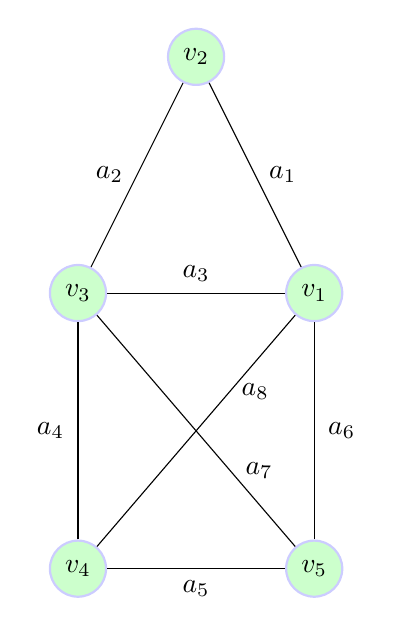
\begin{tikzpicture}{node distance=1.3cm,>=stealth',bend angle=45, auto}
  \tikzstyle{place}=[circle,thick,draw=blue!20,fill=green!20,minimum size=6mm]
  \tikzstyle{texto}=[]

  \begin{scope}

    \node [place] (c1) {$v_1$};

    \node [place] (c2) [above of=c1,xshift=-1.5cm,yshift=2cm] {$v_2$}
    edge [] node [xshift=.35cm] {$a_1$} (c1); 
    
    \node [place] (c3) [left of=c1, xshift=-2cm] {$v_3$}
    edge [] node [yshift=.25cm] {$a_3$} (c1) 
    edge [] node [xshift=-.35cm] {$a_2$} (c2);


    \node [place] (c4) [below of=c3,yshift=-2.5cm] {$v_4$}
    edge [] node [xshift=-.35cm] {$a_4$} (c3) 
    edge [] node [yshift=.5cm,xshift=.75cm] {$a_8$} (c1);

    \node [place] (c5) [below of=c1,yshift=-2.5cm] {$v_5$}
    edge [] node [yshift=-.25cm] {$a_5$} (c4)
    edge [] node [xshift=.35cm] {$a_6$} (c1)
    edge [] node [yshift=-.5cm,xshift=.8cm] {$a_7$} (c3);
\end{scope}  

\end{tikzpicture}
\end{minipage}%
\begin{minipage}{1cm}
\begin{center}
\[
 M =
 \begin{pmatrix}
  0 & 1 & 1 & 1 & 1 \\
  1 & 0 & 1 & 0 & 0 \\
  1 & 1 & 0 & 1 & 1 \\
  1 & 0 & 1 & 0 & 1 \\
  1 & 0 & 1 & 1 & 0 
 \end{pmatrix}
\]
\end{center}
\end{minipage}
\end{figure}%
\end{center}%
\begin{figure}[H]
\begin{center}
\caption{Grafo con su representación en matriz de adyacencia.}%
\end{center}
\end{figure}

Con esta representación, es fácil ver si existe o no una arista entre dos nodos dados: buscar un valor en la matriz requiere un tiempo constante. Por otra parte, si deseamos examinar todos los nodos que estén conectados con algún nodo dado, tenemos que recorrer toda una fila completa de la matriz, en el caso de un grafo no dirigido, o bien tanto una fila completa como una columna completa en el caso de un grafo dirigido. Esto requiere un tiempo que está en $\Theta(V)$, el número de nodos que hay en el grafo, independientemente del número de aristas que entren o salgan de ese nodo particular. El espacio requerido para representar un grafo de esta manera es cuadrático con respecto al número de nodos.\\

La representación por matriz de adyacencia no es satisfactoria para la gran mayoría de grafos dispersos: necesitamos como mínimo para ello $V^2$ bits de almacenamiento y $V^2$ pasos sólo para la construcción de la matriz inicial representativa. En un grafo denso, donde el número de aristas (el número de 1 bit de la matriz) es proporcional a $V^2$, este coste puede ser aceptable, porque el tiempo proporcional a $V^2$ es el necesario para procesar las aristas sin importar la representación que se use en principio. En grafos dispersos, sin embargo, tan sólo la inicialización de la matriz podría ser el factor dominante en el tiempo de ejecución de un algoritmo. Por otra parte, tal vez ni siquiera habría suficiente espacio para la matriz de esa forma. Por ejemplo, podemos estar ante grafos con millones de vértices y decenas de millones de aristas, que sin embargo no tendrán que pagar el precio de reservar espacio en memoria para miles de millones de entradas con el valor 0 en la matriz de adyacencia.\\

Por otro lado, cuando es necesario procesar un grafo denso, las 0-entradas que representan ausencia de arista, incrementan nuestro espacio necesario sólo por un factor constante permitiéndonos determinar así, si cualquiera de las aristas está presente según la constante de tiempo. Si tenemos espacio disponible para almacenar una matriz de adyacencia y si $V^2$ es lo suficientemente pequeño como para ser representado en una cantidad insignificante de tiempo o para hacer uso de un algoritmo complejo que no requiera más de $V^2$ pasos para completarse, la representación mediante matriz de adyacencia puede ser el método de elección adecuado, sin importar lo denso que pueda ser el grafo.\\

\subsection{Matriz de incidencia}

La representación mediante matriz de incidencia de un grafo, es una matriz rectangular $v \times a$ de tantas filas como vértices $v = |V|$ tiene el grafo y tantas columnas como aristas $a = |A|$ hay. La entrada $(i,j)$ consiste en un 1 si el vértice $x_i$ es incidente con la arista $e_j$, siendo 0 en otro caso. Dado que cada arista incide en dos vértices (distintos), esta matriz verifica que cada columna contiene exactamente dos 1, siendo el resto de entradas 0. Toda matriz con esta propiedad es, de hecho, la matriz de incidencia de cierto grafo.

\begin{center}
\[
M = \bordermatrix{~ & a_1 & a_2 & a_3 & a_4 & a_5 & a_6 & a_7 & a_8 \cr
                  v_1 & 1 & 0 & 1 & 0 & 0 & 1 & 0 & 1 \cr
                  v_2 & 1 & 1 & 0 & 0 & 0 & 0 & 0 & 0 \cr
                  v_3 & 0 & 1 & 1 & 1 & 0 & 0 & 1 & 0 \cr
                  v_4 & 0 & 0 & 0 & 1 & 1 & 0 & 0 & 1 \cr
                  v_5 & 0 & 0 & 0 & 0 & 1 & 1 & 1 & 0 \cr}
\]
\end{center}
\begin{figure}[H]
\begin{center}
\caption{Matriz de incidencia del grafo de la Figura 2.10.}
\end{center}
\end{figure}


\subsection{Listas de adyacencia}

La representación estándar preferida para representar grafos que no sean densos es la representación mediante listas de adyacencia, donde hacemos un seguimiento de todos los vértices conectados a cada vértice en una lista enlazada que está asociada con ese vértice. En la lista de adyacencia se asocia a cada nodo i una lista formada por sus vecinos, esto es, una lista formada por aquellos nodos j tales que existe una arista de i a j (en el caso de un grafo dirigido) o entre i e j (en el caso de un grafo no dirigido). Si el número de aristas del grafo es pequeño, esta representación utiliza menos espacio que la dada anteriormente. También puede que sea posible en este caso examinar todos los vecinos de un modo dado en menos de $V$ operaciones de análisis en el caso medio. Por otra parte, determinar si existe o no conexión directa entre dos nodos dados i y j nos obliga a recorrer la lista de vecinos del nodo i (y posiblemente también los del nodo j, en el caso de un grafo dirigido), lo cual es menos eficiente que buscar un valor booleano en una matriz.\\

\begin{center}%
\begin{figure}[H]%
\begin{minipage}[H]{1\columnwidth}%
\centering%
\begin{tikzpicture}{node distance=1.3cm,>=stealth',bend angle=45, auto}
    \matrix [matrix of nodes]
    {
      \node[minimum height=.85cm,draw,tokens=1,yshift=.135cm,label=left:\textcolor{black}{$0$}] (c1) {\ \ \ \ \ \ };&[1cm] \node[minimum height=.7375cm, minimum width=.75cm,draw,yshift=.135cm] (c2) {\ \ \ }; & \node[minimum height=.75cm, minimum width=.75cm,draw] (c3) {\ $6$\ };  &[1cm] \node[minimum height=.7375cm, minimum width=.75cm,draw,yshift=.135cm] (c4) {\ \ \ }; & \node[minimum height=.75cm, minimum width=.75cm,draw] (c5) {\ $5$\ }; & [1cm] \node[minimum height=.7375cm, minimum width=.75cm,draw,yshift=.135cm] (c6) {\ \ \ }; & \node[minimum height=.75cm, minimum width=.75cm,draw] (c7) {\ $1$\ }; & [1cm] \node[minimum height=.7375cm, minimum width=.75cm,draw,yshift=.135cm] (c8) {\ \ \ }; & \node[minimum height=.75cm, minimum width=.75cm,draw] (c9) {\ 2\ };\\
      \node[minimum height=.85cm,draw,tokens=1,yshift=.135cm,label=left:\textcolor{black}{$1$}] (d1) {\ \ \ \ \ \ };&[1cm] \node[minimum height=.7375cm, minimum width=.75cm,draw,yshift=.135cm] (d2) {\ \ \ }; & \node[minimum height=.75cm, minimum width=.75cm,draw] (d3) {\ $0$\ };   \\
      \node[minimum height=.85cm,draw,tokens=1,yshift=.135cm,label=left:\textcolor{black}{$2$}] (e1) {\ \ \ \ \ \ };&[1cm] \node[minimum height=.7375cm, minimum width=.75cm,draw,yshift=.135cm] (e2) {\ \ \ }; & \node[minimum height=.75cm, minimum width=.75cm,draw] (e3) {\ $0$\ };   \\
      \node[minimum height=.85cm,draw,tokens=1,yshift=.135cm,label=left:\textcolor{black}{$3$}] (f1) {\ \ \ \ \ \ }; &[1cm] \node[minimum height=.7375cm, minimum width=.75cm,draw,yshift=.135cm] (f2) {\ \ \ }; & \node[minimum height=.75cm, minimum width=.75cm,draw] (f3) {\ $5$ \ }; &[1cm] \node[minimum height=.7375cm, minimum width=.75cm,draw,yshift=.135cm] (f4) {\ \ \ }; & \node[minimum height=.75cm, minimum width=.75cm,draw] (f5) {\ $4$\ };  \\
      \node[minimum height=.85cm,draw,tokens=1,yshift=.135cm,label=left:\textcolor{black}{$4$}] (g1) {\ \ \ \ \ \ }; &[1cm] \node[minimum height=.7375cm, minimum width=.75cm,draw,yshift=.135cm] (g2) {\ \ \ }; & \node[minimum height=.75cm, minimum width=.75cm,draw] (g3) {\ $6$\ }; &[1cm] \node[minimum height=.7375cm, minimum width=.75cm,draw,yshift=.135cm] (g4) {\ \ \ }; & \node[minimum height=.75cm, minimum width=.75cm,draw] (g5) {\ $5$ \ }; &[1cm] \node[minimum height=.7375cm, minimum width=.75cm,draw,yshift=.135cm] (g6) {\ \ \ }; & \node[minimum height=.75cm, minimum width=.75cm,draw] (g7) {\ $3$ \ };  \\
      \node[minimum height=.85cm,draw,tokens=1,yshift=.135cm,label=left:\textcolor{black}{$5$}] (h1) {\ \ \ \ \ \ }; &[1cm] \node[minimum height=.7375cm, minimum width=.75cm,draw,yshift=.135cm] (h2) {\ \ \ }; & \node[minimum height=.75cm, minimum width=.75cm,draw] (h3) {\ $3$ \ }; &[1cm] \node[minimum height=.7375cm, minimum width=.75cm,draw,yshift=.135cm] (h4) {\ \ \ }; & \node[minimum height=.75cm, minimum width=.75cm,draw] (h5) {\ $0$ \ }; &[1cm] \node[minimum height=.7375cm, minimum width=.75cm,draw,yshift=.135cm] (h6) {\ \ \ }; & \node[minimum height=.75cm, minimum width=.75cm,draw] (h7) {\ $4$ \ };  \\
      \node[minimum height=.85cm,draw,tokens=1,yshift=.135cm,label=left:\textcolor{black}{$6$}] (i1) {\ \ \ \ \ \ }; &[1cm] \node[minimum height=.7375cm, minimum width=.75cm,draw,yshift=.135cm] (i2) {\ \ \ }; & \node[minimum height=.75cm, minimum width=.75cm,draw] (i3) {\ $0$\ }; &[1cm] \node[minimum height=.7375cm, minimum width=.75cm,draw,yshift=.135cm] (i4) {\ \ \ }; & \node[minimum height=.75cm, minimum width=.75cm,draw] (i5) {\ $4$\ };  \\
    };

    \draw (c1) to [post] (c2);
    \draw (c3) to [post] (c4);
    \draw (c5) to [post] (c6);
    \draw (c7) to [post] (c8);
    \draw (d1) to [post] (d2);
    \draw (e1) to [post] (e2);
    \draw (f1) to [post] (f2);
    \draw (f3) to [post] (f4);
    \draw (g1) to [post] (g2);
    \draw (g3) to [post] (g4);
    \draw (g5) to [post] (g6);
    \draw (h1) to [post] (h2);
    \draw (h3) to [post] (h4);
    \draw (h5) to [post] (h6);
    \draw (i1) to [post] (i2);
    \draw (i3) to [post] (i4);

\end{tikzpicture}
\caption{Listas de adyacencia.}%
\end{minipage}%
\end{figure}%
\end{center}%

Para agregar una arista que conecte i e j, se añade j a la lista de adyacencia de i e i a la lista de adyacencia de j. De esta manera, podemos agregar nuevas aristas en tiempo constante, pero la cantidad total de espacio que utilizamos es proporcional al número de vértices más el número de aristas (en comparación con el número de vértices, que formarían un cuadrado en una matriz de adyacencia). Para los grafos no dirigidos, representaremos cada arista en dos lugares distintos: una arista que conecta con i e j se representa con nodos en ambas listas de adyacencia. \\

Con las listas de adyacencia, hay numerosas representaciones de un grafo dado incluso para una determinada numeración de vértices. No importa en qué orden aparezcan las aristas de las listas de adyacencia, ya que la estructura de la lista de adyacencia representará siempre al mismo grafo. Esta característica de las listas de adyacencia es importante para saber porque el orden en que las aristas aparecen en las listas afecta, a su vez, al orden en que las aristas son procesadas por los algoritmos. Es decir, la estructura de las listas de adyacencia determina como se comportará el grafo para el cálculo de un algoritmo sobre él. A pesar de que un algoritmo debe producir una solución correcta sin importar que las aristas estén ordenadas en las listas de adyacencia, se podría llegar a dicha solución por diferentes secuencias de procesamiento del algoritmo sobre diferentes ordenamientos. Si un algoritmo no necesita examinar todas las aristas del grafo para su cálculo, este efecto podría afectar al tiempo de desarrollo del algoritmo. Y, si hay más de una solución correcta, ordenamientos de entrada de aristas diferentes pueden llevar a resultados de salida diferentes.\\

\subsection{Principal ventaja de uso}

La principal ventaja de la representación de listas de adyacencia sobre la representación en matriz de adyacencia es que siempre se utiliza el espacio proporcional a $A + V$, frente a $V^2$ en la matriz de adyacencia. La principal desventaja es que la comprobación de la existencia de arista entre vértices puede llevar un tiempo proporcional a $V$, a diferencia del tiempo constante de la matriz de adyacencia. En estas características, en consecuencia, radica la diferencia entre el uso de listas de adyacencia enlazadas y vectores que representen el conjunto de vértices incidentes con los otros vértices del conjunto. \\

\section{Grados}
\subsection{Grado de un vértice}

\begin{fondo}
Llamaremos grado o valencia de un vértice al número de aristas que incidan en él.
\end{fondo}

Notaremos por $gr_G(v)$ al grado del vértice $v$ en el grafo $G$ y cuando no haya posibilidad de confusión notaremos, simplemente por $gr(v)$.\\

\underline{Algoritmo de comprobación Grado de un vértice}\\
\begin{Verbatim}[commandchars=\\\{\}]
\PY{c+cm}{/**}
\PY{c+cm}{ * Método observador}
\PY{c+cm}{ * @param vertice valor de tipo entero que se corresponde con el vértice}
\PY{c+cm}{ * o nodo del grafo.}
\PY{c+cm}{ * @param G matriz de adyacencia o de costes asociada al grafo.}
\PY{c+cm}{ * @return int: valor entero que se corresponde con la valencia del nodo.}
\PY{c+cm}{ * Número de valencia o grado de un vértice son las aristas }
\PY{c+cm}{ * incidentes en él que contenga.}
\PY{c+cm}{ */}

\PY{k+kd}{public} \PY{k+kt}{int} \PY{n+nf}{grado\PYZus{}vertice}\PY{o}{(}\PY{k+kt}{int} \PY{n}{vertice}\PY{o}{,} \PY{k+kt}{int} \PY{o}{[}\PY{o}{]}\PY{o}{[}\PY{o}{]} \PY{n}{G}\PY{o}{)}
\PY{o}{\PYZob{}}

    \PY{k+kt}{int} \PY{n}{grado}\PY{o}{=}\PY{l+m+mi}{0}\PY{o}{;}
    \PY{k+kt}{int} \PY{n}{tama\PYZus{}G} \PY{o}{=} \PY{n}{G}\PY{o}{.}\PY{n+na}{length}\PY{o}{;}

    \PY{k}{if}\PY{o}{(}\PY{n}{vertice} \PY{o}{<} \PY{l+m+mi}{0} \PY{o}{|}\PY{o}{|} \PY{n}{vertice} \PY{o}{>} \PY{n}{tama\PYZus{}G}\PY{o}{)}
	\PY{o}{\PYZob{}}
	    \PY{n}{System}\PY{o}{.}\PY{n+na}{out}\PY{o}{.}\PY{n+na}{println}\PY{o}{(}\PY{l+s}{"El vértice no esta en el grafo"}\PY{o}{)}\PY{o}{;}
	    \PY{k}{return} \PY{l+m+mi}{0}\PY{o}{;}
	\PY{o}{\PYZcb{}}

    \PY{k}{for}\PY{o}{(}\PY{k+kt}{int} \PY{n}{i}\PY{o}{=}\PY{l+m+mi}{0}\PY{o}{;} \PY{n}{i} \PY{o}{<} \PY{n}{tama\PYZus{}G}\PY{o}{;} \PY{o}{+}\PY{o}{+}\PY{n}{i}\PY{o}{)}
	\PY{o}{\PYZob{}}
	    \PY{k}{if}\PY{o}{(}\PY{n}{G}\PY{o}{[}\PY{n}{vertice}\PY{o}{]}\PY{o}{[}\PY{n}{i}\PY{o}{]} \PY{o}{!}\PY{o}{=} \PY{l+m+mi}{0}\PY{o}{)}
		\PY{n}{grado}\PY{o}{+}\PY{o}{+}\PY{o}{;}
	\PY{o}{\PYZcb{}}

    \PY{k}{return} \PY{n}{grado}\PY{o}{;}
\PY{o}{\PYZcb{}}
\end{Verbatim}


\subsection{Vértice aislado}

\begin{fondo}
Un vértice de grado cero se denomina aislado.
\end{fondo}

\subsection{Suma de los grados de un grafo}
\label{sec:sumagrados}

\begin{fondo}
En cualquier grafo se verifica,
\begin{description}
\item[(a)] La suma de todos sus grados es igual al doble del número de sus aristas.
\item[(b)] El número de vértices de grado impar es par.
\end{description}
\end{fondo}

\figuratikz{1}{Grafo de ejemplo.}
{
  \tikzstyle{place}=[circle,thick,draw=blue!20,fill=green!20,minimum size=6mm]
  \tikzstyle{texto}=[]

  \begin{scope}

    \node [place] (c1) {$v_4$};

    \node [place] (c2) [right of=c1,xshift=1.5cm,yshift=3cm] {$v_3$}
    edge [] (c1);

    \node [place] (c3) [right of=c1,xshift=1.5cm,yshift=-3cm] {$v_5$}
    edge [] (c1)
    edge [] (c2);

    \node [place] (c4) [right of=c2,xshift=3cm] {$v_2$}
    edge [] (c1)
    edge [] (c2)
    edge [] (c3);

    \node [place] (c5) [right of=c3,xshift=3cm] {$v_6$}
    edge [] (c1)
    edge [] (c2)
    edge [] (c3)
    edge [] (c4);

    \node [place] (c6) [above of=c5,yshift=2cm,xshift=2.75cm] {$v_1$}
    edge [] (c1)
    edge [] (c2)
    edge [] (c3)
    edge [] (c4)
    edge [] (c5);

\end{scope}  

}

Sea $G_1 = (V,A)$ siendo\\
\[ V = \{v_1,v_2,v_3,v_4,v_5,v_6\} \]
y\\
\[ A = \{v_1v_2,v_1v_3,v_1v_4,v_1v_5,v_1v_6,v_2v_3,v_2v_4,v_2v_5,v_2v_6,v_3v_4,v_3v_5,v_3v_6,v_4v_5,v_4v_6,v_5v_6\} \]
Entonces, $|A| = 15$ y $gr(v_i) = 5$, $i = 1,2,3,4,5,6$, luego
\[  \sum^{6}_{i=1}{gr(v_i) = 30 = 2 \cdot 15 = 2 |A|} \]
Por otra parte, todos los vértices son de grado impar, luego su número $(6)$ es par.\\

\subsection{Grado de entrada y de salida}

\begin{fondo}
Si $v$ es un vértice de un digrafo $D$, entonces su grado de entrada $gr_e(v)$ es el número de arcos en $D$ de la forma $uv$ y su grado de salida $gr_s(v)$ es el número de arcos en $D$ de la forma $vu$.
\end{fondo}

\section{Isomorfismo}

\subsection{Isomorfismo de grafos}

\begin{fondo}
Dos grafos $G_1 = (V_1,A_1)$ y $G_2 = (V_2,A_2)$ se dice que son isomorfos cuando existe una biyección entre los conjuntos de sus vértices que conserva la adyacencia. Si los grafos $G_1$ y $G_2$ son isomorfos, notaremos $G_1 \simeq G_2$.
\end{fondo}

Según la definición anterior,\\
\[ G_1 \simeq G_2 \iff \exists f\ : V_1 \rightarrow V_2\ : 
\left\{ 
  \begin{array}{l} 
    f\ \mbox{es biyectiva}  \\ 
    uv \in A_1 \iff f(u)(v) \in A_2; \forall u,v \in V_1
  \end{array} 
\right. \]

\figuratikz{1}{Tres grafos isomorfos entre sí.}
{
  \tikzstyle{place}=[circle,thick,draw=blue!20,fill=green!20,minimum size=6mm]
  \tikzstyle{texto}=[]

  \begin{scope}

    \node [place] (c1) {$v_1$};

    \node [place] (c2) [right of=c1,xshift=.4cm] {$v_4$}
    edge [] (c1);

    \node [place] (c3) [right of=c2,yshift=1.2cm] {$v_2$}
    edge [] (c1)
    edge [] (c2);

    \node [place] (c4) [right of=c2,yshift=-1.2cm] {$v_3$}
    edge [] (c1)
    edge [] (c2)
    edge [] (c3);

    \node [place] (c5) [right of=c2,xshift=2cm] {$1$};

    \node [place] (c6) [right of=c5,xshift=1cm,yshift=1.5cm] {$2$}
    edge [] (c5);

    \node [place] (c7) [right of=c5,yshift=-1.5cm] {$4$}
    edge [] (c5)
    edge [] (c6);

    \node [place] (c8) [right of=c5,xshift=1.5cm,yshift=-.5cm] {$3$}
    edge [] (c5)
    edge [] (c6)
    edge [] (c7);

    \node [place] (c9) [right of=c8,xshift=1cm,yshift=.5cm] {$a$};
    
    \node [place] (c10) [right of=c9,xshift=1cm,yshift=1.5cm] {$b$}
    edge [] (c9);

    \node [place] (c11) [right of=c9,yshift=-1.5cm] {$d$}
    edge [] (c9);

    \node [place] (c12) [right of=c9,xshift=1.5cm,yshift=-.5cm] {$c$}
    edge [] (c9)
    edge [] (c10)
    edge [] (c11);

    \draw (c10) .. controls +(-150:2cm) and +(-25:-5cm) .. (c11);

\end{scope}  

}

\section{Subgrafos}

\subsection{Definición}

\begin{fondo}
Un subgrafo de un grafo $G = (V(G),A(G))$ es un grafo $H = (V(H),A(H))$ tal que $V(H) \subseteq V(G)$ y $A(H) \subseteq A(G)$
\end{fondo}

\figuratikz{1}{Un grafo $G$ y tres de sus subgrafos.}
{
  \tikzstyle{place}=[circle,thick,draw=blue!20,fill=green!20,minimum size=6mm]
  \tikzstyle{texto}=[]

  \begin{scope}

    \node [place] (c1) {$v_2$};

    \node [place] (c2) [right of=c1,xshift=1cm] {$v_1$}
    edge [] (c1);

    \node [place] (c3) [below of=c1,yshift=-1cm] {$v_3$}
    edge [] (c1)
    edge [] (c2);

    \node [place] (c4) [below of=c2,yshift=-1cm] {$v_4$}
    edge [] (c1)
    edge [] (c2)
    edge [] (c3);

    \node [texto] (t1) [below of=c3,yshift=.6cm,xshift=1.1cm] {$G$};

    \node [place] (c5) [right of=c2,xshift=.5cm] {$v_2$};

    \node [place] (c6) [right of=c5,xshift=1cm] {$v_1$}
    edge [] (c5);

    \node [place] (c7) [below of=c6,yshift=-1cm] {$v_4$}
    edge [] (c5)
    edge [] (c6);

    \node [texto] (t2) [below of=c7,yshift=.6cm,xshift=-1.2cm] {$H_1$};

    \node [place] (c8) [right of=c6,xshift=.5cm]{$v_2$};

    \node [place] (c9) [right of=c8,xshift=1cm] {$v_1$}
    edge [] (c8);

    \node [place] (c10) [below of=c8,yshift=-1cm] {$v_3$};

    \node [place] (c11) [below of=c9,yshift=-1cm] {$v_4$}
    edge [] (c8)
    edge [] (c9);

    \node [texto] (t3) [below of=c10,yshift=.6cm,xshift=1.1cm] {$H_2$};
    
    \node [place] (c12) [right of=c9,xshift=.5cm]{$v_2$};

    \node [texto] (c13) [right of=c12,xshift=1cm] {};

    \node [place] (c14) [below of=c12,yshift=-1cm] {$v_3$}
    edge [] (c12);

    \node [place] (c15) [below of=c13,yshift=-1cm] {$v_4$}
    edge [] (c14);

    \node [texto] (t4) [below of=c14,yshift=.6cm,xshift=1.1cm] {$H_3$};

\end{scope}  

}
\[G = \{v_1,v_2,v_3,v_4\},\{v_1v_2,v_1v_3,v_1v_4,v_2v_3,v_2v_4,v_3v_4\}\]
\[H_1 = \{v_1,v_2,v_4\},\{v_1v_2,v_1v_4,v_2v_4\}\]
\[H_2 = \{v_1,v_2,v_3,v_4\},\{v_1v_2,v_1v_4,v_2v_4\}\]
\[H_3 = \{v_2,v_3,v_4\},\{v_2v_3,v_3v_4\}\]
\subsection{Eliminación de aristas}

\begin{fondo}
Si $a$ es una arista del grafo $G$, entonces el subgrafo $G \setminus \{a\}$ es el grafo que se obtiene de $G$ eliminando la arista $a$.\\
En general, escribiremos $G \setminus \{a_1,a_2, \ldots, a_k\}$ para denominar al subgrafo que se obtiene de $G$ eliminando las aristas $a_1,a_2, \ldots, a_k$.
\end{fondo}

\subsection{Eliminación de vértices}

\begin{fondo}
Si $v$ es un vértice del grafo $G$, entonces el subgrafo $G \setminus \{v\}$ es el grafo que se obtiene de $G$ eliminando el vértice $v$.\\
En general, escribiremos $G \setminus \{v_1,v_2, \ldots, v_k\}$ para denominar al subgrafo que se obtiene de $G$ eliminando los vértices $v_1,v_2, \ldots, v_k$.
\end{fondo}

\section{Caminos y ciclos}

\subsection{Camino}

\begin{fondo}
Sea $G$ un grafo o un multigrafo. Un camino en $G$ es una sucesión donde se alternan vértices y aristas, comenzando y terminando con vértices y en el que cada arista es incidente con los dos vértices que la preceden y la siguen.
\end{fondo}

Un camino que une los vértices $v_1$ y $v_n$ sería:\\
\[v_1, v_1v_2, v_2, v_2v_3, \ldots, v_{n-1}, v_{n-1}v_n, v_n \]
Si se trata de un grafo (no un multigrafo) este camino también puede especificarse simplemente por la sucesión de sus vértices, $v_1, v_2, v_3, \ldots, v_{n-1}, v_n$ y lo representamos por:\\
\[ \gamma = \langle v_1, v_2, v_3, \ldots, v_{n-1}, v_n \rangle \]
A los vértices $v_1$ y $v_n$ se les denomina extremos del camino. Suele decirse también que el camino conecta $v_1$ con $v_n$ o que va de $v_1$ a $v_n$. La longitud del camino es el número $n-1$ de aristas que contiene. Un camino es simple si en la sucesión de vértices no hay ninguno repetido. \\

\subsection{Ciclo}

\begin{fondo}
Sea $G$ un grafo o un multigrafo. Un ciclo en $G$ es un camino en el que sus extremos coinciden.\\

El ciclo será simple si no hay, además del primero y el último, ningún otro vértice repetido.
\end{fondo}

\figuratikz{1}{Caminos y ciclos.}
{
  \tikzstyle{place}=[circle,thick,draw=blue!20,fill=green!20,minimum size=6mm]
  \tikzstyle{texto}=[]

  \begin{scope}

    \node [place] (c1) {$v_5$};

    \node [place] (c2) [right of=c1,xshift=.5cm,yshift=3cm] {$v_4$};

    \node [place] (c3) [above of=c2,xshift=3cm] {$v_3$};

    \node [place] (c4) [right of=c1,xshift=3.5cm] {$v_6$};

    \node [place] (c5) [right of=c2,xshift=4.5cm] {$v_2$};

    \node [place] (c6) [right of=c4,xshift=3.5cm] {$v_1$};

    %\draw (c1) .. controls +(50:-2cm) and +(10:1cm) .. (c2);

    \draw (c1) .. controls +(-80:-2cm) and +(-100:2cm) .. (c2);
    \draw (c1) .. controls +(-10:1cm) and +(-10:-3cm) .. (c4);
    \draw (c2) .. controls +(10:1cm) and +(-10:-2cm) .. (c3);
    \draw (c2) .. controls +(-10:1cm) and +(-30:-1cm) .. (c4);
    \draw (c3) .. controls +(-60:2cm) and +(-70:-3cm) .. (c4);
    \draw (c3) .. controls +(-180:-1cm) and +(5:-1cm) .. (c5);
    \draw (c5) .. controls +(-150:2cm) and +(40:1cm) .. (c4);
    \draw (c5) .. controls +(-70:2cm) and +(150:1cm) .. (c6);

\end{scope}  

}

\quad $\gamma = \langle v_1,\ v_2,\ v_6,\ v_3,\ v_4,\ v_6,\ v_5 \rangle$ es un camino.\\

\quad $\gamma = \langle v_1,\ v_2,\ v_3,\ v_4 \rangle$ es un camino simple ya que no hay ningún vértice repetido.\\

\quad $\gamma = \langle v_1,\ v_2,\ v_6,\ v_5,\ v_4,\ v_6,\ v_2,\ v_1 \rangle$ es un ciclo.\\

\quad $\gamma = \langle v_2,\ v_3,\ v_4,\ v_5,\ v_6,\ v_2 \rangle$ es un ciclo simple ya que se repiten, únicamente, los \hspace*{.15in}{vértices primero y último.}\\


Un grafo acíclico no contiene ningún ciclo. Los árboles están conectados con los grafos no dirigidos acíclicos. Los árboles son los grafos más simples, y sus estructuras intrínsecamente recursivas, ya que la eliminación o corte de cualesquieras aristas deja como resultado dos pequeños árboles.

A los grafos dirigidos acíclicos se les llaman DAG. Estos surgen de forma natural en los problemas de horarios, donde una arista dirigida $(x,y)$ indica que la actividad de $x$ debe ocurrir antes que $y$. Una operación llamada \emph{ordenación topológica} ordena los vértices de un DAG según restricciones de precedencia en la ejecución o procesamiento de dichos elementos. La ordenación topológica es típicamente el primer paso para cualquier algoritmo sobre un DAG.

\begin{nota}
Se muestra una aproximación de comprobación de Aciclicidad para grafo dirigidos.\\
\end{nota}

\underline{Algoritmo de Comprobación de Aciclicidad}\\
\begin{Verbatim}[commandchars=\\\{\}]
\PY{c+cm}{/**}
\PY{c+cm}{ * Método observador. (para grafos dirigidos)}
\PY{c+cm}{ * Comprueba si un grafo dirigido es aciclico o no.}
\PY{c+cm}{ * @param G array multidimensional (matriz) que contiene la matriz}
\PY{c+cm}{ * de adyacencia del grafo G asociado.}
\PY{c+cm}{ * @return devuelve true o false (verdadero o falso) si se cumple}
\PY{c+cm}{ * que sea o no acíclico.}
\PY{c+cm}{ */}

\PY{k+kd}{public} \PY{k+kt}{boolean} \PY{n+nf}{AciclicoGD}\PY{o}{(}\PY{k+kt}{int} \PY{o}{[}\PY{o}{]}\PY{o}{[}\PY{o}{]} \PY{n}{G}\PY{o}{)}
\PY{o}{\PYZob{}}
	
    \PY{k+kt}{int} \PY{n}{tama\PYZus{}G} \PY{o}{=} \PY{n}{G}\PY{o}{.}\PY{n+na}{length}\PY{o}{;}
    \PY{k+kt}{int} \PY{n}{i}\PY{o}{;}
    \PY{k+kt}{boolean} \PY{n}{aciclico} \PY{o}{=} \PY{k+kc}{true}\PY{o}{;} 
    \PY{c+c1}{// El grafo es acíclico hasta que se demuestre lo contrario.}
    \PY{n}{visitados} \PY{o}{=} \PY{k}{new} \PY{k+kt}{boolean}\PY{o}{[}\PY{n}{tama\PYZus{}G}\PY{o}{]}\PY{o}{;}
    \PY{n}{ancestros} \PY{o}{=} \PY{k}{new} \PY{k+kt}{int}\PY{o}{[}\PY{n}{tama\PYZus{}G}\PY{o}{]}\PY{o}{;}
    \PY{c+c1}{// Para llevar la cuenta de los ancestros.}

    \PY{c+c1}{// Al comienzo no hay ningún vértice visitado.}
    \PY{n}{Arrays}\PY{o}{.}\PY{n+na}{fill}\PY{o}{(}\PY{n}{visitados}\PY{o}{,} \PY{k+kc}{false}\PY{o}{)}\PY{o}{;}

    \PY{c+cm}{/* Vamos iterando de componente en componente conexa}
\PY{c+cm}{       para sacar el árbol de expansión */}

    \PY{k}{for}\PY{o}{(}\PY{n}{i}\PY{o}{=}\PY{l+m+mi}{0}\PY{o}{;} \PY{n}{i} \PY{o}{<} \PY{n}{tama\PYZus{}G} \PY{o}{&}\PY{o}{&} \PY{n}{aciclico} \PY{o}{=}\PY{o}{=} \PY{k+kc}{true}\PY{o}{;} \PY{o}{+}\PY{o}{+}\PY{n}{i}\PY{o}{)}
	\PY{o}{\PYZob{}}
	    \PY{k}{if}\PY{o}{(}\PY{o}{!}\PY{n}{visitados}\PY{o}{[}\PY{n}{i}\PY{o}{]}\PY{o}{)}
		\PY{n}{aciclico} \PY{o}{=} \PY{n}{AciclicoGDRec}\PY{o}{(}\PY{n}{i}\PY{o}{,}\PY{n}{G}\PY{o}{,}\PY{l+m+mi}{0}\PY{o}{)}\PY{o}{;}
	\PY{o}{\PYZcb{}}
	
    \PY{k}{return} \PY{n}{aciclico}\PY{o}{;}
\PY{o}{\PYZcb{}}

\PY{c+cm}{/**}
\PY{c+cm}{ * Función privada de la clase que sirve para iterar sobre la estructura}
\PY{c+cm}{ * de aristas del grafo.}
\PY{c+cm}{ * @param vertice vértice inicial desde el que se realiza la búsqueda }
\PY{c+cm}{ * en el grafo.}
\PY{c+cm}{ * @param G array multidimensional (matriz) que contiene la matriz}
\PY{c+cm}{ * de adyacencia del grafo G asociado.}
\PY{c+cm}{ * @param num\PYZus{}ancestros número de vértices visitados anteriormente desde }
\PY{c+cm}{ * el vértice de partida.}
\PY{c+cm}{ * @return devuelve true o false (verdadero o falso) dependiendo de si }
\PY{c+cm}{ * encuentra un ciclo o no en la estructura.}
\PY{c+cm}{ */}

\PY{k+kd}{private} \PY{k+kt}{boolean} \PY{n+nf}{AciclicoGDRec}\PY{o}{(}\PY{k+kt}{int} \PY{n}{vertice}\PY{o}{,} \PY{k+kt}{int} \PY{o}{[}\PY{o}{]}\PY{o}{[}\PY{o}{]} \PY{n}{G}\PY{o}{,} \PY{k+kt}{int} \PY{n}{num\PYZus{}ancestros}\PY{o}{)} 
\PY{o}{\PYZob{}}
    \PY{k+kt}{int} \PY{n}{w}\PY{o}{=}\PY{l+m+mi}{0}\PY{o}{;}
    \PY{c+c1}{// Para movernos por los vértices adyacentes.}

    \PY{k+kt}{int} \PY{n}{i}\PY{o}{;}
    \PY{c+c1}{// Para movernos por los ancestros.}

    \PY{n}{visitados}\PY{o}{[}\PY{n}{vertice}\PY{o}{]} \PY{o}{=} \PY{k+kc}{true}\PY{o}{;}
    \PY{c+c1}{// Acabamos de visitar dicho vértice.}

    \PY{n}{ancestros}\PY{o}{[}\PY{n}{num\PYZus{}ancestros}\PY{o}{]} \PY{o}{=} \PY{n}{vertice}\PY{o}{;}
    \PY{c+c1}{// Guardamos el ancestro.}
	

    \PY{c+cm}{/* Ahora recorremos todos los vértices y miramos cuales son}
\PY{c+cm}{       adyacentes y de ellos los que no hemos visitado. Con estos}
\PY{c+cm}{       vértices seguimos la búsqueda en profundidad. */}

    \PY{k}{for}\PY{o}{(}\PY{n}{w}\PY{o}{=}\PY{l+m+mi}{0}\PY{o}{;} \PY{n}{w} \PY{o}{<} \PY{n}{G}\PY{o}{[}\PY{n}{vertice}\PY{o}{]}\PY{o}{[}\PY{n}{w}\PY{o}{]}\PY{o}{;} \PY{o}{+}\PY{o}{+}\PY{n}{w}\PY{o}{)}
	\PY{o}{\PYZob{}}
	    \PY{k}{if}\PY{o}{(}\PY{n}{G}\PY{o}{[}\PY{n}{vertice}\PY{o}{]}\PY{o}{[}\PY{n}{w}\PY{o}{]} \PY{o}{!}\PY{o}{=} \PY{l+m+mi}{0}\PY{o}{)}
		\PY{o}{\PYZob{}}
		    \PY{k}{if}\PY{o}{(}\PY{o}{!}\PY{n}{visitados}\PY{o}{[}\PY{n}{w}\PY{o}{]}\PY{o}{)}
			\PY{k}{return} \PY{o}{(}\PY{n}{AciclicoGDRec}\PY{o}{(}\PY{n}{w}\PY{o}{,}\PY{n}{G}\PY{o}{,}\PY{n}{num\PYZus{}ancestros}\PY{o}{+}\PY{o}{+}\PY{o}{)}\PY{o}{)}\PY{o}{;}
		    \PY{k}{else}
			\PY{o}{\PYZob{}}
			    \PY{c+c1}{// Si el vértice ya se ha visitado.}
			    \PY{k}{for}\PY{o}{(}\PY{n}{i}\PY{o}{=}\PY{l+m+mi}{0}\PY{o}{;} \PY{n}{i} \PY{o}{<}\PY{o}{=} \PY{n}{num\PYZus{}ancestros}\PY{o}{;} \PY{o}{+}\PY{o}{+}\PY{n}{i}\PY{o}{)}
				\PY{o}{\PYZob{}}
				    \PY{c+c1}{// Lo encontramos hay una arista.}
				    \PY{k}{if}\PY{o}{(}\PY{n}{ancestros}\PY{o}{[}\PY{n}{i}\PY{o}{]} \PY{o}{=}\PY{o}{=} \PY{n}{w}\PY{o}{)}
					\PY{k}{return} \PY{o}{(}\PY{k+kc}{false}\PY{o}{)}\PY{o}{;} \PY{c+c1}{//Hay un ciclo.}
					
				\PY{o}{\PYZcb{}}
			\PY{o}{\PYZcb{}}
		\PY{o}{\PYZcb{}}
	\PY{o}{\PYZcb{}}
	
    \PY{k}{return} \PY{o}{(}\PY{k+kc}{true}\PY{o}{)}\PY{o}{;} \PY{c+c1}{// Si llegamos aquí no se habrá encontrado ningún ciclo.}
\PY{o}{\PYZcb{}}
\end{Verbatim}


\section{Conexión en grafos}

Una de las propiedades más elementales de las que puede gozar cualquier grafo es que sea conexo.

\subsection{Vértices conectados}

\begin{fondo}
Dos vértices de un grafo se dice que están conectados cuando existe un camino entre ambos. Es decir,
\begin{center}$u$ y $v$ están conectados $\iff$ $\exists \mu = \langle u, v \rangle$ \end{center}
$\mu$ es un camino que une al vértice $u$ con el $v$.
\end{fondo}

\subsection{Grafos conexos}

\begin{fondo}
Un grafo se dice que es conexo si cada par de sus vértices están conectados. Es decir,
\begin{center} $G$ es conexo $\iff$ $\forall u, v$ : $\exists \mu = \langle u, v \rangle$ \end{center}
En caso contrario, diremos que $G$ es un grafo desconexo.
\end{fondo}

\figuratikz{1}{Ejemplos de grafos conexos.}
{
  \tikzstyle{place}=[circle,thick,draw=blue!20,fill=green!20,minimum size=6mm]
  \tikzstyle{texto}=[]

  \begin{scope}

    \node [place] (c1) {$v_1$};

    \node [place] (c2) [right of=c1,xshift=1cm] {$v_2$}
    edge [] (c1);

    \node [place] (c3) [above of=c2,xshift=1cm] {$v_3$}
    edge [] (c2);

    \node [place] (c4) [right of=c3,yshift=-1cm,xshift=1cm] {$v_4$}
    edge [] (c3);

    \node [place] (c5) [below of=c3,xshift=.5cm] {$v_5$}
    edge [] (c4)
    edge [] (c3);

    \node [texto] (t1) [below of=c2,xshift=.7cm,yshift=.3cm] {Grafo conexo $G_1$};

    \node [place] (c6) [right of=c5,xshift=3cm] {$v_1$};

    \node [place] (c7) [right of=c6,xshift=1cm] {$v_2$}
    edge [] (c6);

    \node [place] (c8) [above of=c7,xshift=1cm] {$v_3$};

    \node [place] (c9) [right of=c8,yshift=-1cm,xshift=1cm] {$v_4$}
    edge [] (c8);

    \node [place] (c10) [below of=c8,xshift=.5cm] {$v_5$}
    edge [] (c9)
    edge [] (c8);

    \node [texto] (t2) [below of=c7,xshift=.7cm,yshift=.3cm] {Grafo desconexo $G_2$};


\end{scope}  

}

\subsection{Proposición}

\begin{fondo}
Dado un grafo, la relación ``estar conectado con'' definida en el conjunto de sus vértices es una relación de equivalencia.
\end{fondo}

\underline{Demostración}\\

Sea el grafo $G = (V,A)$ y definimos el conjunto $V$ de sus vértices la siguiente relación
\[ u {\cal{R}} v \iff u\ \mbox{está conectado con}\ v\]
Veamos que esta relación es de equivalencia.\\
\begin{description}
\item[(a)]\emph{Reflexividad}. Sea $u$ cualquiera de $V$. Entonces, el camino $\mu = \langle u, u \rangle$ conecta $u$ con \\ \hspace*{-.1in}{$u$, luego}
\[ \forall u \in V\ ; u {\cal{R}} u \]
\hspace*{-.1in}{es decir $\cal R$ es reflexiva.}
\item[(b)]\emph{Simetría}. Sea $u$ y $v$ dos elementos cualesquiera de $V$. Entonces,
\[ u {\cal{R}} v \iff \exists \mu = \langle u, v \rangle \Longrightarrow \exists \mu' = \langle v, u \rangle \iff v {\cal{R}} u \]
\hspace*{-.1in}{luego,}
\[ \forall u, v \in V ; u {\cal{R}} v \Longrightarrow v {\cal{R}} u \]
\hspace*{-.1in}{o sea, $\cal{R}$ es simétrica.}
\item[(c)]\emph{Transitividad}. Si $u,v$ y $w$ son tres vértices cualesquiera de $G$, entonces
\[
  \begin{array}{l}
    u {\cal{R}} v \iff \exists \mu_1 = \langle u, v \rangle \\
    v {\cal{R}} w \iff \exists \mu_2 = \langle v, w \rangle \\
  \end{array}
  \Biggl\} \Longrightarrow \exists \mu = \langle u, w \rangle \iff u {\cal{R}} w
\]
\hspace*{-.1in}{Bastaría, pues, con unir los caminos $\mu_1$ y $\mu_2$. Por lo tanto}
\[ \forall u, v, w ; u {\cal{R}} v \land v {\cal{R}} w \Longrightarrow u {\cal{R}} w \]
\hspace*{-.1in}{es decir, $\cal{R}$ es transitiva.}
\end{description}

\subsection{Componentes conexas de un grafo}

\begin{fondo}
Dado un grafo $G = (V,A)$, las clases de equivalencia en el conjunto de sus vértices, $V$, por la relación de equivalencia ``estar conectado con'' reciben el nombre de componentes conexas de $G$.
\end{fondo}

Obsérvese que de esta forma un grafo no conexo G puede ser ``partido'' por la relación anterior en subgrafos conexos que son las citadas componentes conexas de $G$.

\begin{ejem}
El conjunto de vértices del grafo $G_2$ de la figura 2.17 es
\[V = \{v_1, v_2, v_3, v_4, v_5 \} \]
y si consideramos en él la relación de equivalencia definida en la proposición anterior, las clases de equivalencia serán
\[ [v_1] = \{v_1, v_2\} = [v_2] \]
\[ [v_3] = \{v_3, v_4, v_5\} = [v_4] = [v_5] \]
Por lo tanto, el grafo $G_2$ tiene dos componentes conexas que son los subgrafos $H_1$ y $H_2$ cuyos conjuntos de vértices son $[v_1]$ y $[v_3]$, es decir,
\[ H_1 = (\{v_1, v_2\}, \{v_1v_2\}) \]
\[ H_2 = (\{v_3, v_4, v_5\}, \{v_3v_4, v_3v_5, v_4v_5\}) \]
\\
\end{ejem}

\begin{ejem}
Demostraremos que en un grafo conexo $G = (V,A)$ se verifica: $|V| - 1 \leq |A|$\\
\end{ejem}

\underline{Solución}

Utilizaremos la inducción sobre el número de vértices de $G$.

\emph{Paso básico.} Si $|V| = 1$, entonces $|A| = 0$, luego
\[ |V| - 1 = 1 - 1 = 0 = |A| \]

\emph{Paso inductivo.} Supongamos que la desigualdad es cierta para $|V| = p$ con $p > 1$ y veamos que también es cierta para $|V| = p + 1$.\\

En efecto, sea $u$ un vértice cualquier de $G$. Como el número de vértices, $p$, es mayor que 1, habrá otro vértice, $v$ en $G$ distinto de $u$ y, al ser $G$ conexo, deberá existir, al menos, un camino entre $u$ y $v$, luego $gr(v) \ge 1$.\\

\begin{itemize}
\item Si $gr(u) = 1$ y $a$ es la única arista que tiene a $u$ como extremo, entonces el grafo
\[(V \setminus \{u\}, A \setminus \{a\})\]
es conexo y tiene $p$ vértices. Por la hipótesis de inducción,\\
\[ |V \setminus \{u\}| -1 \leq |A \setminus \{a\}| \]
es decir,
\[ |V| - 2 \leq |A| -1 \]
de donde,
\[ |V| - 1 \leq |A| \]
\item Si $gr(u) > 1$, $\forall u \in V$, entonces por el teorema \ref{sec:sumagrados}
\[ 2|V| \leq \mbox{Suma de los grados de los vértices de}\ G = 2|A| \]
o sea, $|V| \leq |A|$, de aquí que
\[ |V| - 1 < |A| \]
Por el \emph{primer principio de inducción matemática},
\[ |V| - 1 \leq |A| \]
\end{itemize}

\subsection{Puntos de corte}

\begin{fondo}
Dado un grafo conexo $G = (V,A)$, un vértice $u$ de $G$ se llama punto de corte cuando el subgrafo $G_u$ cuyos vértices son los de $V \setminus \{u\}$ y cuyas aristas son todas las de $A$ cuyos vértices están en $V \setminus \{u\}$ no es conexo.
\end{fondo}

Una consecuencia de esto es que uno de los conjuntos de corte produce exactamente dos componentes.\\

A veces es útil para indicar un conjunto límite fijado por la partición de los vértices que induce. Si $V$ denota al conjunto de vértices de $G$ y si $P$ es el subconjunto de vértices en una componente de $G$ inducida por el conjunto o punto de corte, entonces el límite del conjunto se puede especificar por $(P,\overline P)$ donde $\overline P = V - P$.\\

\begin{nota}
El algoritmo implementado verifica si existe algún punto de corte en el grafo. Hay otra versión que muestra dichos puntos de cortes del grafo.\\
\end{nota}

\underline{Algoritmo Comprobación Puntos de Corte}\\
\begin{Verbatim}[commandchars=\\\{\}]
\PY{c+cm}{/**}
\PY{c+cm}{ * Algoritmo de comprobación de vértices de corte - Método modificador.}
\PY{c+cm}{ * Muestra por la salida estándar los nodos de corte del grafo.}
\PY{c+cm}{ * @return boolean: representa un valor lógico que indica si se ha encontrado}
\PY{c+cm}{ * un punto de corte(true) o no(false) en el grafo.}
\PY{c+cm}{ * @exception Exception}
\PY{c+cm}{ */}

\PY{k+kd}{public} \PY{k+kt}{boolean} \PY{n+nf}{vertice\PYZus{}corte}\PY{o}{(}\PY{o}{)} \PY{k+kd}{throws} \PY{n}{Exception}
\PY{o}{\PYZob{}}
    \PY{n}{System}\PY{o}{.}\PY{n+na}{out}\PY{o}{.}\PY{n+na}{println}\PY{o}{(}\PY{l+s}{"Se procede a la búsqueda de vértice de corte"}\PY{o}{)}\PY{o}{;}
    \PY{n}{array\PYZus{}grados}\PY{o}{(}\PY{o}{)}\PY{o}{;}

    \PY{k+kt}{int} \PY{n}{tama\PYZus{}G} \PY{o}{=} \PY{k}{this}\PY{o}{.}\PY{n+na}{devolver\PYZus{}matriz}\PY{o}{(}\PY{o}{)}\PY{o}{.}\PY{n+na}{length}\PY{o}{;}
    \PY{k+kt}{int} \PY{n}{aux}\PY{o}{=}\PY{l+m+mi}{0}\PY{o}{;}
    \PY{k+kt}{boolean} \PY{n}{punto\PYZus{}corte}\PY{o}{=}\PY{k+kc}{true}\PY{o}{;}

    \PY{k}{for}\PY{o}{(}\PY{k+kt}{int} \PY{n}{i}\PY{o}{=}\PY{l+m+mi}{0}\PY{o}{;} \PY{n}{i} \PY{o}{<} \PY{n}{tama\PYZus{}G}\PY{o}{;} \PY{o}{+}\PY{o}{+}\PY{n}{i}\PY{o}{)}
	\PY{o}{\PYZob{}}
	    \PY{n}{aux} \PY{o}{=} \PY{n}{grados\PYZus{}interno}\PY{o}{.}\PY{n+na}{get}\PY{o}{(}\PY{n}{i}\PY{o}{)}\PY{o}{;}
	    \PY{k}{if}\PY{o}{(}\PY{k}{this}\PY{o}{.}\PY{n+na}{n\PYZus{}aristas}\PY{o}{(}\PY{o}{)} \PY{o}{-} \PY{n}{aux} \PY{o}{<} \PY{o}{(}\PY{k}{this}\PY{o}{.}\PY{n+na}{n\PYZus{}nodos}\PY{o}{(}\PY{o}{)} \PY{o}{-} \PY{l+m+mi}{1}\PY{o}{)}\PY{o}{)}
		\PY{n}{punto\PYZus{}corte} \PY{o}{=} \PY{k+kc}{false}\PY{o}{;}
	\PY{o}{\PYZcb{}}

    \PY{k}{return} \PY{n}{punto\PYZus{}corte}\PY{o}{;}
\PY{o}{\PYZcb{}}
\end{Verbatim}


\subsection{Puentes}

\begin{fondo}
Dado un grafo conexo $G = (V,A)$, a cualquier arista ``$a$'' de $G$ tal que el grafo $(V, A \setminus \{a\})$ no sea conexo, lo llamaremos puente.
\end{fondo}

\figuratikzno{1}{}{}
{
  \tikzstyle{place}=[circle,thick,draw=blue!20,fill=green!20,minimum size=6mm]
  \tikzstyle{texto}=[]

  \begin{scope}

    \node [place] (c1) {$v_6$};

    \node [place] (c2) [right of=c1,xshift=1cm,yshift=2.5cm] {$v_5$}
    edge [] (c1);

    \node [place] (c3) [right of=c1,xshift=1cm,yshift=-2.5cm] {$v_7$}
    edge [] (c1)
    edge [] (c2);

    \node [place] (c4) [right of=c2,xshift=2cm] {$v_4$}
    edge [] (c2);

    \node [place] (c5) [right of=c3,xshift=2cm] {$v_8$}
    edge [] (c4);

    \node [place] (c6) [right of=c1,xshift=6cm] {$v_3$}
    edge [] (c4)
    edge [] (c5);

    \node [place] (c7) [right of=c4,xshift=2.5cm] {$v_2$}
    edge [] (c6);

    \node [place] (c8) [right of=c5,xshift=2.5cm] {$v_9$}
    edge [] (c6);

    \node [place] (c9) [right of=c6,xshift=1.75cm] {$v_1$}
    edge [] (c7)
    edge [] (c8);

    \node [texto] (t1) [below of=c5,yshift=.2cm] {$G$};
\end{scope}  

}

Puntos de corte. Los vértices $v_3, v_4$ y $v_5$ ya que en la figura existen puntos que no pueden conectarse a través de ningún camino.\\

Puentes. El único puente que existe en el grafo propuesto es la arista $v_4v_5$ ya que en el grafo resultante existen vértices que no están conectados, es decir, no es conexo.\\
\begin{fondo}
Si $G = (V,A)$ es un grafo conexo y $a$ es una arista puente de $G$, entonces $(V,A \setminus \{a\})$ tiene exactamente dos componentes conexas.
\end{fondo}

\underline{Demostración}\\

Llamemos $v$ y $w$ a los vértices que son extremos de la arista $a$. Y dividamos los vértices de $G$ en dos clases:
\begin{enumerate}
\item El conjunto de vértices $V_1$, formado por aquellos para los que existe un camino que los conecta con $v$ \emph{sin usar} la arista $a$ (esto es, sin pasar por el vértice $w$). Entre estos está, por supuesto, el propio vértice $v$.
\item El conjunto de vértices $V_2$ de los vértices que \emph{necesariamente} han de usar la arista $a$ para conectarse a $v$. Entre ello está $w$.
\end{enumerate}

Que esto es una partición de los vértices de $G$ es obvio. Pero, además, la intersección de $V_1$ y $V_2$ es vacía: si un vértice $x \in V$ estuviera en $V_1$ y en $V_2$ a la vez, $a$ no sería arista puente, porque podríamos quitarla sin que se desconectara el grafo. Si ahora formamos el grafo $G = (V, A \setminus \{a\})$, sus dos componentes conexas son, precisamente, los vértices de $V_1$ (y sus aristas) y los vértices de $V_2$ (y sus aristas).\\

\underline{Algoritmo comprobación de Puentes}\\
\begin{Verbatim}[commandchars=\\\{\}]
\PY{c+cm}{/**}
\PY{c+cm}{ * Método modificador}
\PY{c+cm}{ * Método que halla las aristas de corte (puentes) de un grafo.}
\PY{c+cm}{ * @param G: matriz bidimensional de enteros que representa el grafo de}
\PY{c+cm}{ * trabajo actual.}
\PY{c+cm}{ */}

\PY{k+kd}{public} \PY{k+kt}{void} \PY{n+nf}{puentes}\PY{o}{(}\PY{k+kt}{int} \PY{o}{[}\PY{o}{]}\PY{o}{[}\PY{o}{]} \PY{n}{G}\PY{o}{)}
\PY{o}{\PYZob{}}
    \PY{k+kt}{int} \PY{n}{tama\PYZus{}G} \PY{o}{=} \PY{n}{G}\PY{o}{.}\PY{n+na}{length}\PY{o}{;}
    \PY{n}{hash\PYZus{}puentes} \PY{o}{=} \PY{k}{new} \PY{n}{HashMap}\PY{o}{<}\PY{n}{Integer}\PY{o}{,}\PY{n}{ArrayList}\PY{o}{<}\PY{n}{Integer}\PY{o}{>}\PY{o}{>}\PY{o}{(}\PY{o}{)}\PY{o}{;}
    \PY{n}{ArrayList}\PY{o}{<}\PY{n}{Integer}\PY{o}{>} \PY{n}{array\PYZus{}puentes}\PY{o}{;}
    \PY{n}{ArrayList}\PY{o}{<}\PY{n}{Arista}\PY{o}{>} \PY{n}{bridge} \PY{o}{=} \PY{k}{new} \PY{n}{ArrayList}\PY{o}{<}\PY{n}{Arista}\PY{o}{>}\PY{o}{(}\PY{o}{)}\PY{o}{;}
    \PY{n}{Arista} \PY{n}{I\PYZus{}J}\PY{o}{;}

    \PY{n}{grado\PYZus{}vector}\PY{o}{(}\PY{n}{G}\PY{o}{)}\PY{o}{;}
    \PY{k+kt}{boolean} \PY{n}{siguiente}\PY{o}{;}

    \PY{k}{for}\PY{o}{(}\PY{k+kt}{int} \PY{n}{i}\PY{o}{=}\PY{l+m+mi}{0}\PY{o}{;} \PY{n}{i} \PY{o}{<} \PY{n}{tama\PYZus{}G}\PY{o}{;} \PY{o}{+}\PY{o}{+}\PY{n}{i}\PY{o}{)}
	\PY{o}{\PYZob{}}
	    \PY{n}{array\PYZus{}puentes} \PY{o}{=} \PY{k}{new} \PY{n}{ArrayList}\PY{o}{<}\PY{n}{Integer}\PY{o}{>}\PY{o}{(}\PY{o}{)}\PY{o}{;}
		
	    \PY{k}{for}\PY{o}{(}\PY{k+kt}{int} \PY{n}{j}\PY{o}{=}\PY{l+m+mi}{0}\PY{o}{;} \PY{n}{j} \PY{o}{<} \PY{n}{tama\PYZus{}G}\PY{o}{;} \PY{o}{+}\PY{o}{+}\PY{n}{j}\PY{o}{)}
		\PY{o}{\PYZob{}}
		    \PY{k}{if}\PY{o}{(}\PY{n}{G}\PY{o}{[}\PY{n}{i}\PY{o}{]}\PY{o}{[}\PY{n}{j}\PY{o}{]} \PY{o}{!}\PY{o}{=} \PY{l+m+mi}{0}\PY{o}{)}
			\PY{n}{array\PYZus{}puentes}\PY{o}{.}\PY{n+na}{add}\PY{o}{(}\PY{n}{j}\PY{o}{)}\PY{o}{;}
		\PY{o}{\PYZcb{}}

	    \PY{n}{hash\PYZus{}puentes}\PY{o}{.}\PY{n+na}{put}\PY{o}{(}\PY{n}{i}\PY{o}{,}\PY{n}{array\PYZus{}puentes}\PY{o}{)}\PY{o}{;}

	\PY{o}{\PYZcb{}}
	
	
    \PY{k}{for}\PY{o}{(}\PY{k+kt}{int} \PY{n}{i}\PY{o}{=}\PY{l+m+mi}{0}\PY{o}{;} \PY{n}{i} \PY{o}{<} \PY{n}{tama\PYZus{}G}\PY{o}{;} \PY{o}{+}\PY{o}{+}\PY{n}{i}\PY{o}{)}
	\PY{k}{for}\PY{o}{(}\PY{k+kt}{int} \PY{n}{j}\PY{o}{=}\PY{l+m+mi}{0}\PY{o}{;} \PY{n}{j} \PY{o}{<} \PY{n}{hash\PYZus{}puentes}\PY{o}{.}\PY{n+na}{get}\PY{o}{(}\PY{n}{i}\PY{o}{)}\PY{o}{.}\PY{n+na}{size}\PY{o}{(}\PY{o}{)}\PY{o}{;} \PY{o}{+}\PY{o}{+}\PY{n}{j}\PY{o}{)}
	    \PY{o}{\PYZob{}}

		\PY{n}{I\PYZus{}J} \PY{o}{=} \PY{k}{new} \PY{n}{Arista}\PY{o}{(}\PY{o}{)}\PY{o}{;}
		\PY{n}{siguiente} \PY{o}{=} \PY{k+kc}{true}\PY{o}{;}

		\PY{k}{if}\PY{o}{(}\PY{n}{bridge}\PY{o}{.}\PY{n+na}{size}\PY{o}{(}\PY{o}{)} \PY{o}{!}\PY{o}{=} \PY{l+m+mi}{0}\PY{o}{)}
		    \PY{o}{\PYZob{}}
			\PY{k}{if}\PY{o}{(}\PY{n}{i} \PY{o}{=}\PY{o}{=} \PY{n}{bridge}\PY{o}{.}\PY{n+na}{get}\PY{o}{(}\PY{l+m+mi}{0}\PY{o}{)}\PY{o}{.}\PY{n+na}{v\PYZus{}destino}\PY{o}{(}\PY{o}{)} 
			   \PY{o}{&}\PY{o}{&} \PY{n}{hash\PYZus{}puentes}\PY{o}{.}\PY{n+na}{get}\PY{o}{(}\PY{n}{i}\PY{o}{)}\PY{o}{.}\PY{n+na}{get}\PY{o}{(}\PY{n}{j}\PY{o}{)} 
			   \PY{o}{=}\PY{o}{=} \PY{n}{bridge}\PY{o}{.}\PY{n+na}{get}\PY{o}{(}\PY{l+m+mi}{0}\PY{o}{)}\PY{o}{.}\PY{n+na}{v\PYZus{}origen}\PY{o}{(}\PY{o}{)}\PY{o}{)} 
			    \PY{o}{\PYZob{}}
				\PY{n}{siguiente} \PY{o}{=} \PY{k+kc}{false}\PY{o}{;}
				\PY{n}{bridge}\PY{o}{.}\PY{n+na}{remove}\PY{o}{(}\PY{l+m+mi}{0}\PY{o}{)}\PY{o}{;}
			    \PY{o}{\PYZcb{}}
				
		    \PY{o}{\PYZcb{}}

		\PY{k}{if}\PY{o}{(}\PY{n}{siguiente}\PY{o}{)}
		    \PY{k}{if}\PY{o}{(}\PY{n}{puentes\PYZus{}rec}\PY{o}{(}\PY{n}{i}\PY{o}{,}\PY{n}{hash\PYZus{}puentes}\PY{o}{.}\PY{n+na}{get}\PY{o}{(}\PY{n}{i}\PY{o}{)}\PY{o}{.}\PY{n+na}{get}\PY{o}{(}\PY{n}{j}\PY{o}{)}\PY{o}{,}\PY{n}{tama\PYZus{}G}\PY{o}{)}\PY{o}{)}
			\PY{o}{\PYZob{}}
			    \PY{n}{System}\PY{o}{.}\PY{n+na}{out}\PY{o}{.}\PY{n+na}{println}\PY{o}{(}\PY{l+s}{"Puente en: i:"}\PY{o}{+}\PY{n}{i}\PY{o}{+}\PY{l+s}{" j:"}
					       \PY{o}{+}\PY{n}{hash\PYZus{}puentes}\PY{o}{.}\PY{n+na}{get}\PY{o}{(}\PY{n}{i}\PY{o}{)}\PY{o}{.}\PY{n+na}{get}\PY{o}{(}\PY{n}{j}\PY{o}{)}\PY{o}{)}\PY{o}{;}
			    \PY{n}{I\PYZus{}J}\PY{o}{.}\PY{n+na}{v\PYZus{}origen}\PY{o}{(}\PY{n}{i}\PY{o}{)}\PY{o}{;}
			    \PY{n}{I\PYZus{}J}\PY{o}{.}\PY{n+na}{v\PYZus{}destino}\PY{o}{(}\PY{n}{hash\PYZus{}puentes}\PY{o}{.}\PY{n+na}{get}\PY{o}{(}\PY{n}{i}\PY{o}{)}\PY{o}{.}\PY{n+na}{get}\PY{o}{(}\PY{n}{j}\PY{o}{)}\PY{o}{)}\PY{o}{;}
			    \PY{n}{I\PYZus{}J}\PY{o}{.}\PY{n+na}{coste}\PY{o}{(}\PY{l+m+mi}{0}\PY{o}{)}\PY{o}{;}
			    \PY{n}{bridge}\PY{o}{.}\PY{n+na}{add}\PY{o}{(}\PY{n}{I\PYZus{}J}\PY{o}{)}\PY{o}{;}
			\PY{o}{\PYZcb{}}
	    \PY{o}{\PYZcb{}}	

\PY{o}{\PYZcb{}}

\PY{c+cm}{/**}
\PY{c+cm}{ * Método observador. (privado)}
\PY{c+cm}{ * Método recursivo que ayuda a la ejecución de la llamada principal de }
\PY{c+cm}{ * puentes. Comprueba si existe un puente para la arista de entrada como}
\PY{c+cm}{ * parámetro formal formada por sus vértices.}
\PY{c+cm}{ * @param u: valor entero que representa un extremo de la arista.}
\PY{c+cm}{ * @param v: valor entero que representa el otro extremo de la arista.}
\PY{c+cm}{ * @param tama\PYZus{}G: valor entero que representa el número de nodos del grafo.}
\PY{c+cm}{ * @return boolean: devolverá true o false dependiendo de si la arista}
\PY{c+cm}{ * es una arista de corte (puente) o no.}
\PY{c+cm}{ */}

\PY{k+kd}{private} \PY{k+kt}{boolean} \PY{n+nf}{puentes\PYZus{}rec}\PY{o}{(}\PY{k+kt}{int} \PY{n}{u}\PY{o}{,} \PY{k+kt}{int} \PY{n}{v}\PY{o}{,} \PY{k+kt}{int} \PY{n}{tama\PYZus{}G}\PY{o}{)}
\PY{o}{\PYZob{}}
    \PY{k+kt}{int} \PY{n}{pos\PYZus{}valencia}\PY{o}{=}\PY{l+m+mi}{0}\PY{o}{;}
    \PY{k+kt}{boolean} \PY{n}{camino}\PY{o}{=}\PY{k+kc}{false}\PY{o}{;}
    \PY{k+kt}{boolean} \PY{n}{fin}\PY{o}{=}\PY{k+kc}{false}\PY{o}{;}


    \PY{k+kt}{int} \PY{n}{i}\PY{o}{=}\PY{n}{u}\PY{o}{;}
    \PY{k+kt}{int} \PY{n}{ant\PYZus{}u}\PY{o}{=}\PY{n}{u}\PY{o}{;}
    \PY{k+kt}{int} \PY{n}{ant\PYZus{}v}\PY{o}{=}\PY{n}{v}\PY{o}{;} \PY{c+c1}{//Almacenamos los vértices origen.}

    \PY{n}{ArrayList}\PY{o}{<}\PY{n}{Integer}\PY{o}{>} \PY{n}{vertice\PYZus{}i} \PY{o}{=} \PY{k}{new} \PY{n}{ArrayList}\PY{o}{<}\PY{n}{Integer}\PY{o}{>}\PY{o}{(}\PY{o}{)}\PY{o}{;}
    \PY{n}{ArrayList}\PY{o}{<}\PY{n}{Integer}\PY{o}{>} \PY{n}{vertice\PYZus{}j} \PY{o}{=} \PY{k}{new} \PY{n}{ArrayList}\PY{o}{<}\PY{n}{Integer}\PY{o}{>}\PY{o}{(}\PY{o}{)}\PY{o}{;}

    \PY{k}{while}\PY{o}{(}\PY{o}{!}\PY{n}{fin}\PY{o}{)}
	\PY{o}{\PYZob{}}
	    \PY{c+cm}{/* Primero insertamos los nodos adyacentes de vertice\PYZus{}i (u)}
\PY{c+cm}{	       y luego hacemos lo mismo para los nodos adyacentes de}
\PY{c+cm}{	       vertice\PYZus{}j (v). Por ello cuando cambiemos los valores serán}
\PY{c+cm}{	       iteraciones pares (vertice\PYZus{}i) o impares (vertice\PYZus{}j).}
\PY{c+cm}{	    */}

	    \PY{k}{if}\PY{o}{(}\PY{n}{pos\PYZus{}valencia} \PY{o}{\PYZpc{}} \PY{l+m+mi}{2} \PY{o}{=}\PY{o}{=} \PY{l+m+mi}{0}\PY{o}{)}
		\PY{o}{\PYZob{}}

		    \PY{k}{if}\PY{o}{(}\PY{n}{vertice\PYZus{}i}\PY{o}{.}\PY{n+na}{size}\PY{o}{(}\PY{o}{)} \PY{o}{!}\PY{o}{=} \PY{l+m+mi}{0}\PY{o}{)}
			\PY{o}{\PYZob{}}
			    \PY{n}{ant\PYZus{}u} \PY{o}{=} \PY{n}{ant\PYZus{}v}\PY{o}{;}
			    \PY{n}{i} \PY{o}{=} \PY{n}{vertice\PYZus{}i}\PY{o}{.}\PY{n+na}{get}\PY{o}{(}\PY{l+m+mi}{0}\PY{o}{)}\PY{o}{;}
			    \PY{n}{vertice\PYZus{}i}\PY{o}{.}\PY{n+na}{remove}\PY{o}{(}\PY{l+m+mi}{0}\PY{o}{)}\PY{o}{;}


			    \PY{k}{for}\PY{o}{(}\PY{k+kt}{int} \PY{n}{j}\PY{o}{=}\PY{l+m+mi}{0}\PY{o}{;} \PY{n}{j} \PY{o}{<} \PY{n}{hash\PYZus{}puentes}\PY{o}{.}\PY{n+na}{get}\PY{o}{(}\PY{n}{i}\PY{o}{)}\PY{o}{.}\PY{n+na}{size}\PY{o}{(}\PY{o}{)}\PY{o}{;} \PY{o}{+}\PY{o}{+}\PY{n}{j}\PY{o}{)}
				\PY{o}{\PYZob{}}
				    \PY{c+cm}{/* En la primera estructura metemos }
\PY{c+cm}{				       los adyacentes del nodo u de la }
\PY{c+cm}{				       arista (u,v) */}

				    \PY{k}{if}\PY{o}{(}\PY{n}{hash\PYZus{}puentes}\PY{o}{.}\PY{n+na}{get}\PY{o}{(}\PY{n}{i}\PY{o}{)}\PY{o}{.}\PY{n+na}{get}\PY{o}{(}\PY{n}{j}\PY{o}{)} \PY{o}{!}\PY{o}{=} \PY{n}{ant\PYZus{}u}\PY{o}{)}
					\PY{n}{vertice\PYZus{}i}\PY{o}{.}\PY{n+na}{add}\PY{o}{(}\PY{n}{hash\PYZus{}puentes}\PY{o}{.}\PY{n+na}{get}\PY{o}{(}\PY{n}{i}\PY{o}{)}\PY{o}{.}\PY{n+na}{get}\PY{o}{(}\PY{n}{j}\PY{o}{)}\PY{o}{)}\PY{o}{;}
				\PY{o}{\PYZcb{}}
			\PY{o}{\PYZcb{}}
		    \PY{k}{else}\PY{o}{\PYZob{}}

			\PY{k}{if}\PY{o}{(}\PY{n}{hash\PYZus{}puentes}\PY{o}{.}\PY{n+na}{get}\PY{o}{(}\PY{n}{i}\PY{o}{)}\PY{o}{.}\PY{n+na}{size}\PY{o}{(}\PY{o}{)} \PY{o}{=}\PY{o}{=} \PY{l+m+mi}{1} 
			   \PY{o}{&}\PY{o}{&} \PY{n}{hash\PYZus{}puentes}\PY{o}{.}\PY{n+na}{get}\PY{o}{(}\PY{n}{i}\PY{o}{)}\PY{o}{.}\PY{n+na}{get}\PY{o}{(}\PY{l+m+mi}{0}\PY{o}{)} \PY{o}{=}\PY{o}{=} \PY{n}{v}\PY{o}{)}
			    \PY{o}{\PYZob{}}
				\PY{n}{fin} \PY{o}{=} \PY{k+kc}{true}\PY{o}{;}
				\PY{n}{camino} \PY{o}{=} \PY{k+kc}{true}\PY{o}{;}
			    \PY{o}{\PYZcb{}}

			\PY{k}{for}\PY{o}{(}\PY{k+kt}{int} \PY{n}{j}\PY{o}{=}\PY{l+m+mi}{0}\PY{o}{;} \PY{n}{j} \PY{o}{<} \PY{n}{hash\PYZus{}puentes}\PY{o}{.}\PY{n+na}{get}\PY{o}{(}\PY{n}{i}\PY{o}{)}\PY{o}{.}\PY{n+na}{size}\PY{o}{(}\PY{o}{)}\PY{o}{;} \PY{o}{+}\PY{o}{+}\PY{n}{j}\PY{o}{)}
			    \PY{o}{\PYZob{}}
				\PY{c+cm}{/* En la primera estructura metemos los }
\PY{c+cm}{				   adyacentes del nodo u de la arista (u,v) */}
	
				\PY{k}{if}\PY{o}{(}\PY{n}{hash\PYZus{}puentes}\PY{o}{.}\PY{n+na}{get}\PY{o}{(}\PY{n}{i}\PY{o}{)}\PY{o}{.}\PY{n+na}{get}\PY{o}{(}\PY{n}{j}\PY{o}{)} \PY{o}{!}\PY{o}{=} \PY{n}{v}\PY{o}{)}
				    \PY{n}{vertice\PYZus{}i}\PY{o}{.}\PY{n+na}{add}\PY{o}{(}\PY{n}{hash\PYZus{}puentes}\PY{o}{.}\PY{n+na}{get}\PY{o}{(}\PY{n}{i}\PY{o}{)}\PY{o}{.}\PY{n+na}{get}\PY{o}{(}\PY{n}{j}\PY{o}{)}\PY{o}{)}\PY{o}{;}
			    \PY{o}{\PYZcb{}}\PY{o}{\PYZcb{}}


		\PY{o}{\PYZcb{}}

	    \PY{k}{if}\PY{o}{(}\PY{n}{pos\PYZus{}valencia} \PY{o}{\PYZpc{}} \PY{l+m+mi}{2} \PY{o}{!}\PY{o}{=} \PY{l+m+mi}{0}\PY{o}{)}
		\PY{o}{\PYZob{}}
		    \PY{k}{if}\PY{o}{(}\PY{n}{vertice\PYZus{}j}\PY{o}{.}\PY{n+na}{size}\PY{o}{(}\PY{o}{)} \PY{o}{!}\PY{o}{=} \PY{l+m+mi}{0}\PY{o}{)}
			\PY{o}{\PYZob{}}
			    \PY{n}{ant\PYZus{}v} \PY{o}{=} \PY{n}{ant\PYZus{}u}\PY{o}{;}
			    \PY{n}{v} \PY{o}{=} \PY{n}{vertice\PYZus{}j}\PY{o}{.}\PY{n+na}{get}\PY{o}{(}\PY{l+m+mi}{0}\PY{o}{)}\PY{o}{;}
			    \PY{n}{vertice\PYZus{}j}\PY{o}{.}\PY{n+na}{remove}\PY{o}{(}\PY{l+m+mi}{0}\PY{o}{)}\PY{o}{;}
				
			    \PY{k}{for}\PY{o}{(}\PY{k+kt}{int} \PY{n}{j}\PY{o}{=}\PY{l+m+mi}{0}\PY{o}{;} \PY{n}{j} \PY{o}{<} \PY{n}{hash\PYZus{}puentes}\PY{o}{.}\PY{n+na}{get}\PY{o}{(}\PY{n}{v}\PY{o}{)}\PY{o}{.}\PY{n+na}{size}\PY{o}{(}\PY{o}{)}\PY{o}{;} \PY{o}{+}\PY{o}{+}\PY{n}{j}\PY{o}{)}
				\PY{o}{\PYZob{}}
				    \PY{c+cm}{/* En la segunda estructura metemos }
\PY{c+cm}{				       los adyacentes del nodo v de la }
\PY{c+cm}{				       arista (u,v) */}
		
				    \PY{k}{if}\PY{o}{(}\PY{n}{hash\PYZus{}puentes}\PY{o}{.}\PY{n+na}{get}\PY{o}{(}\PY{n}{v}\PY{o}{)}\PY{o}{.}\PY{n+na}{get}\PY{o}{(}\PY{n}{j}\PY{o}{)} \PY{o}{!}\PY{o}{=} \PY{n}{ant\PYZus{}v}\PY{o}{)}			    
					\PY{n}{vertice\PYZus{}j}\PY{o}{.}\PY{n+na}{add}\PY{o}{(}\PY{n}{hash\PYZus{}puentes}\PY{o}{.}\PY{n+na}{get}\PY{o}{(}\PY{n}{v}\PY{o}{)}\PY{o}{.}\PY{n+na}{get}\PY{o}{(}\PY{n}{j}\PY{o}{)}\PY{o}{)}\PY{o}{;}
					
				\PY{o}{\PYZcb{}}
				
			\PY{o}{\PYZcb{}}
		    \PY{k}{else}
			\PY{o}{\PYZob{}}


			    \PY{k}{if}\PY{o}{(}\PY{n}{hash\PYZus{}puentes}\PY{o}{.}\PY{n+na}{get}\PY{o}{(}\PY{n}{v}\PY{o}{)}\PY{o}{.}\PY{n+na}{size}\PY{o}{(}\PY{o}{)} \PY{o}{=}\PY{o}{=} \PY{l+m+mi}{1} 
			       \PY{o}{&}\PY{o}{&} \PY{n}{hash\PYZus{}puentes}\PY{o}{.}\PY{n+na}{get}\PY{o}{(}\PY{n}{v}\PY{o}{)}\PY{o}{.}\PY{n+na}{get}\PY{o}{(}\PY{l+m+mi}{0}\PY{o}{)} \PY{o}{=}\PY{o}{=} \PY{n}{u}\PY{o}{)}
				\PY{o}{\PYZob{}}
				    \PY{n}{fin} \PY{o}{=} \PY{k+kc}{true}\PY{o}{;}
				    \PY{n}{camino} \PY{o}{=} \PY{k+kc}{true}\PY{o}{;}
				\PY{o}{\PYZcb{}}

				    
			    \PY{k}{for}\PY{o}{(}\PY{k+kt}{int} \PY{n}{j}\PY{o}{=}\PY{l+m+mi}{0}\PY{o}{;} \PY{n}{j} \PY{o}{<} \PY{n}{hash\PYZus{}puentes}\PY{o}{.}\PY{n+na}{get}\PY{o}{(}\PY{n}{v}\PY{o}{)}\PY{o}{.}\PY{n+na}{size}\PY{o}{(}\PY{o}{)}\PY{o}{;} \PY{o}{+}\PY{o}{+}\PY{n}{j}\PY{o}{)}
				\PY{o}{\PYZob{}}
				    \PY{c+cm}{/* En la segunda estructura metemos }
\PY{c+cm}{				       los adyacentes del nodo}
\PY{c+cm}{				       v de la arista (u,v)*/}
					
				    \PY{k}{if}\PY{o}{(}\PY{n}{hash\PYZus{}puentes}\PY{o}{.}\PY{n+na}{get}\PY{o}{(}\PY{n}{v}\PY{o}{)}\PY{o}{.}\PY{n+na}{get}\PY{o}{(}\PY{n}{j}\PY{o}{)} \PY{o}{!}\PY{o}{=} \PY{n}{u}\PY{o}{)}			    
					\PY{n}{vertice\PYZus{}j}\PY{o}{.}\PY{n+na}{add}\PY{o}{(}\PY{n}{hash\PYZus{}puentes}\PY{o}{.}\PY{n+na}{get}\PY{o}{(}\PY{n}{v}\PY{o}{)}\PY{o}{.}\PY{n+na}{get}\PY{o}{(}\PY{n}{j}\PY{o}{)}\PY{o}{)}\PY{o}{;}
					
				\PY{o}{\PYZcb{}}
			\PY{o}{\PYZcb{}}
		\PY{o}{\PYZcb{}}
		
	    \PY{k}{for}\PY{o}{(}\PY{k+kt}{int} \PY{n}{j}\PY{o}{=}\PY{l+m+mi}{0}\PY{o}{;} \PY{n}{j} \PY{o}{<} \PY{n}{vertice\PYZus{}i}\PY{o}{.}\PY{n+na}{size}\PY{o}{(}\PY{o}{)} \PY{o}{&}\PY{o}{&} \PY{o}{!}\PY{n}{camino}\PY{o}{;} \PY{o}{+}\PY{o}{+}\PY{n}{j}\PY{o}{)}
		\PY{k}{for}\PY{o}{(}\PY{k+kt}{int} \PY{n}{k}\PY{o}{=}\PY{l+m+mi}{0}\PY{o}{;} \PY{n}{k} \PY{o}{<} \PY{n}{vertice\PYZus{}j}\PY{o}{.}\PY{n+na}{size}\PY{o}{(}\PY{o}{)} \PY{o}{&}\PY{o}{&} \PY{o}{!}\PY{n}{camino}\PY{o}{;} \PY{o}{+}\PY{o}{+}\PY{n}{k}\PY{o}{)}
		    \PY{o}{\PYZob{}}
		
			\PY{k}{if}\PY{o}{(}\PY{n}{vertice\PYZus{}i}\PY{o}{.}\PY{n+na}{get}\PY{o}{(}\PY{n}{j}\PY{o}{)} \PY{o}{=}\PY{o}{=} \PY{n}{vertice\PYZus{}j}\PY{o}{.}\PY{n+na}{get}\PY{o}{(}\PY{n}{k}\PY{o}{)}\PY{o}{)}
			    \PY{o}{\PYZob{}}
				\PY{c+cm}{/* Al llegar a este caso significa}
\PY{c+cm}{				   que se ha recorrido todo los nodos}
\PY{c+cm}{				   adyacentes posibles y no se ha hallado}
\PY{c+cm}{				   ningún camino auxiliar que conecte}
\PY{c+cm}{				   u y v. Por tanto (u,v) es una arista}
\PY{c+cm}{				   de corte.}
\PY{c+cm}{				*/}

				\PY{n}{camino} \PY{o}{=} \PY{k+kc}{false}\PY{o}{;}
				\PY{n}{fin} \PY{o}{=} \PY{k+kc}{true}\PY{o}{;}
			    \PY{o}{\PYZcb{}}
		    \PY{o}{\PYZcb{}}
	
	    \PY{n}{pos\PYZus{}valencia}\PY{o}{+}\PY{o}{+}\PY{o}{;}

	    \PY{k}{if}\PY{o}{(}\PY{n}{vertice\PYZus{}i}\PY{o}{.}\PY{n+na}{size}\PY{o}{(}\PY{o}{)} \PY{o}{=}\PY{o}{=} \PY{l+m+mi}{2}\PY{o}{)}
		\PY{k}{if}\PY{o}{(}\PY{n}{vertice\PYZus{}i}\PY{o}{.}\PY{n+na}{get}\PY{o}{(}\PY{l+m+mi}{0}\PY{o}{)} \PY{o}{=}\PY{o}{=} \PY{n}{vertice\PYZus{}i}\PY{o}{.}\PY{n+na}{get}\PY{o}{(}\PY{l+m+mi}{1}\PY{o}{)}\PY{o}{)}
		    \PY{o}{\PYZob{}}
			\PY{c+cm}{/* Al llegar a este caso significa}
\PY{c+cm}{			   que se ha encontrado un camino }
\PY{c+cm}{			   secundario para la arista (u,v),}
\PY{c+cm}{			   que conectaría los nodos u y v */}

			\PY{n}{fin} \PY{o}{=} \PY{k+kc}{true}\PY{o}{;}
			\PY{n}{camino} \PY{o}{=} \PY{k+kc}{true}\PY{o}{;}
		    \PY{o}{\PYZcb{}}

	    \PY{k}{if}\PY{o}{(}\PY{n}{vertice\PYZus{}j}\PY{o}{.}\PY{n+na}{size}\PY{o}{(}\PY{o}{)} \PY{o}{=}\PY{o}{=} \PY{l+m+mi}{2}\PY{o}{)}
		\PY{k}{if}\PY{o}{(}\PY{n}{vertice\PYZus{}j}\PY{o}{.}\PY{n+na}{get}\PY{o}{(}\PY{l+m+mi}{0}\PY{o}{)} \PY{o}{=}\PY{o}{=} \PY{n}{vertice\PYZus{}j}\PY{o}{.}\PY{n+na}{get}\PY{o}{(}\PY{l+m+mi}{1}\PY{o}{)}\PY{o}{)}
		    \PY{o}{\PYZob{}}
			\PY{c+cm}{/* Al llegar a este caso significa}
\PY{c+cm}{			   que se ha encontrado un camino }
\PY{c+cm}{			   secundario para la arista (u,v),}
\PY{c+cm}{			   que conectaría los nodos u y v */}

			\PY{n}{fin} \PY{o}{=} \PY{k+kc}{true}\PY{o}{;}
			\PY{n}{camino} \PY{o}{=} \PY{k+kc}{true}\PY{o}{;}
		    \PY{o}{\PYZcb{}}
	\PY{o}{\PYZcb{}}
    \PY{k}{return} \PY{n}{camino}\PY{o}{;}
		
\PY{o}{\PYZcb{}}
\end{Verbatim}



\section{Estructura de partición}

Una partición de un conjunto $C$ de elementos de un cierto tipo es un conjunto de subconjuntos disjuntos cuya unión es el conjunto total $C$.\\
Esta estructura se ha adaptado, en este caso, para representar particiones de elementos del tipo Arista cuyo representación interna es de la forma:
\[ Arista\ a\ =\ \langle x,y,z \rangle:
\left\{ 
\begin{array}{l}
x\ \mbox{el vértice origen}\\
y\ \mbox{el vértice destino}\\
z\ \mbox{el coste de la arista} 
\end{array}
\right. \]

Una relación de equivalencia sobre los elementos de un conjunto $C$ define una partición $C$ y, viceversa, cualquier partición de $C$ define una relación de equivalencia sobre sus elementos, de tal forma que cada miembro de la partición es una clase de equivalencia. Así pues, para cada subconjunto o clase podemos elegir cualquier elemento como representante canónico de todos sus miembros.\\

A continuación se da la especificación del TAD que representará la estructura de partición de nuestro sistema:\\

\underline{TAD Partición}\\
\begin{Verbatim}[commandchars=\\\{\}]
\PY{k+kd}{public} \PY{k+kd}{class} \PY{n+nc}{Particion}
\PY{o}{\PYZob{}}

    \PY{c+cm}{/**}
\PY{c+cm}{     * Atributos privados}
\PY{c+cm}{     */}

    \PY{c+cm}{/*}
\PY{c+cm}{      Array de enteros que contiene los padres}
\PY{c+cm}{      de las posiciones (nodos) del sistema.}
\PY{c+cm}{    */}

    \PY{k+kd}{private} \PY{k+kt}{int} \PY{o}{[}\PY{o}{]} \PY{n}{padre}\PY{o}{;}

    \PY{c+cm}{/*}
\PY{c+cm}{      Valor entero que cuyo contenido es}
\PY{c+cm}{      el número de nodos que posee el grafo.}
\PY{c+cm}{    */}

    \PY{k+kd}{private} \PY{k+kt}{int} \PY{n}{nEltos}\PY{o}{;}

    \PY{c+cm}{/**}
\PY{c+cm}{     * Constructor nulo.}
\PY{c+cm}{     */}

    \PY{k+kd}{public} \PY{n+nf}{Particion}\PY{o}{(}\PY{o}{)} \PY{o}{\PYZob{}}\PY{o}{\PYZcb{}}

    \PY{c+cm}{/**}
\PY{c+cm}{     * Constructor predeterminado.}
\PY{c+cm}{     * Se implementa un bosque de árboles (con control de altura). }
\PY{c+cm}{     * Compresión de caminos.}
\PY{c+cm}{     * @param n número de elementos de la partición que se crea}
\PY{c+cm}{     */}

    \PY{k+kd}{public} \PY{n+nf}{Particion}\PY{o}{(}\PY{k+kt}{int} \PY{n}{n}\PY{o}{)}
    \PY{o}{\PYZob{}}
	\PY{n}{padre} \PY{o}{=} \PY{k}{new} \PY{k+kt}{int}\PY{o}{[}\PY{n}{n}\PY{o}{]}\PY{o}{;}
	\PY{n}{nEltos} \PY{o}{=} \PY{n}{n}\PY{o}{;}

	\PY{n}{Arrays}\PY{o}{.}\PY{n+na}{fill}\PY{o}{(}\PY{n}{padre}\PY{o}{,}\PY{l+m+mi}{0}\PY{o}{,}\PY{n}{nEltos}\PY{o}{,}\PY{o}{-}\PY{l+m+mi}{1}\PY{o}{)}\PY{o}{;}
	\PY{c+c1}{//Creamos n árboles de altura 0 representada con -1}
    \PY{o}{\PYZcb{}}

    \PY{c+cm}{/**}
\PY{c+cm}{     * Método modificador.}
\PY{c+cm}{     * Une el subconjunto del elemento a y el del elemento b en uno }
\PY{c+cm}{     * de los subconjuntos arbitrariamente. La partición P queda }
\PY{c+cm}{     * con un miembro menos.}
\PY{c+cm}{     * @param a representante de la clase de partición (nodo).}
\PY{c+cm}{     * @param b representante de la clase de partición (nodo).}
\PY{c+cm}{     * @return void}
\PY{c+cm}{     */}
    
    \PY{k+kd}{public} \PY{k+kt}{void} \PY{n+nf}{Union}\PY{o}{(}\PY{k+kt}{int} \PY{n}{a}\PY{o}{,} \PY{k+kt}{int} \PY{n}{b}\PY{o}{)}
    \PY{o}{\PYZob{}}
	\PY{k}{if}\PY{o}{(}\PY{n}{padre}\PY{o}{[}\PY{n}{b}\PY{o}{]} \PY{o}{<} \PY{n}{padre}\PY{o}{[}\PY{n}{a}\PY{o}{]}\PY{o}{)}
	    \PY{n}{padre}\PY{o}{[}\PY{n}{a}\PY{o}{]} \PY{o}{=} \PY{n}{b}\PY{o}{;}
	\PY{k}{else}
	    \PY{o}{\PYZob{}}
	 	\PY{k}{if}\PY{o}{(}\PY{n}{padre}\PY{o}{[}\PY{n}{a}\PY{o}{]} \PY{o}{=}\PY{o}{=} \PY{n}{padre}\PY{o}{[}\PY{n}{b}\PY{o}{]}\PY{o}{)}
	 	    \PY{n}{padre}\PY{o}{[}\PY{n}{a}\PY{o}{]}\PY{o}{-}\PY{o}{-}\PY{o}{;}

	 	\PY{n}{padre}\PY{o}{[}\PY{n}{b}\PY{o}{]} \PY{o}{=} \PY{n}{a}\PY{o}{;}
	    \PY{o}{\PYZcb{}}
    \PY{o}{\PYZcb{}}

    \PY{c+cm}{/**}
\PY{c+cm}{     * Método observador.}
\PY{c+cm}{     * Devuelve el representante del subconjunto al que }
\PY{c+cm}{     * pertenece el elemento x.}
\PY{c+cm}{     * @param x elemento de la partición.}
\PY{c+cm}{     * @return devuelve el representante del subconjunto }
\PY{c+cm}{     * al que pertenece el elemento x.}
\PY{c+cm}{     */}

    \PY{k+kd}{public} \PY{k+kt}{int} \PY{n+nf}{Encontrar}\PY{o}{(}\PY{k+kt}{int} \PY{n}{x}\PY{o}{)}
    \PY{o}{\PYZob{}}
	\PY{k+kt}{int} \PY{n}{raiz}\PY{o}{,}\PY{n}{y}\PY{o}{;}

	\PY{n}{raiz} \PY{o}{=} \PY{n}{x}\PY{o}{;}

	\PY{k}{while}\PY{o}{(}\PY{n}{padre}\PY{o}{[}\PY{n}{raiz}\PY{o}{]} \PY{o}{>} \PY{o}{-}\PY{l+m+mi}{1}\PY{o}{)}
	    \PY{n}{raiz} \PY{o}{=} \PY{n}{padre}\PY{o}{[}\PY{n}{raiz}\PY{o}{]}\PY{o}{;}

	\PY{c+cm}{/* Los nodos del camino de x a raiz se hacen }
\PY{c+cm}{	   hijo de raiz. */}
	
	\PY{k}{while}\PY{o}{(}\PY{n}{padre}\PY{o}{[}\PY{n}{x}\PY{o}{]} \PY{o}{>}\PY{o}{=} \PY{n}{raiz}\PY{o}{)}
	    \PY{o}{\PYZob{}}
	 	\PY{n}{y} \PY{o}{=} \PY{n}{padre}\PY{o}{[}\PY{n}{x}\PY{o}{]}\PY{o}{;}
	 	\PY{n}{padre}\PY{o}{[}\PY{n}{x}\PY{o}{]} \PY{o}{=} \PY{n}{raiz}\PY{o}{;}
	 	\PY{n}{x} \PY{o}{=} \PY{n}{y}\PY{o}{;}
	    \PY{o}{\PYZcb{}}

	\PY{k}{return} \PY{n}{raiz}\PY{o}{;}
    \PY{o}{\PYZcb{}}

    
\PY{o}{\PYZcb{}}
\end{Verbatim}


La estructura de datos alternativa que se ha usado para la implementación de ciertas operaciones del TAD ha sido la de Bosque de Árboles. \\

La causa por la que operación \emph{Unión()} no se ejecuta en un tiempo constante es que para cada elemento se almacena el representante de su clase y esto obliga a modificar el representante de todos los elementos de uno de los conjuntos unidos. Podemos cambiar la estructura de datos para conseguir que la unión sea $O(1)$, pero a costa de empeorar el tiempo de ejecución de la operación \emph{Encontrar()}, ya que no existe una estructura de datos que permita ejecutar simultáneamente estas dos operaciones en un tiempo constante.\\

\vspace{-.3in}{\section{Disperso frente a denso}

Se define la densidad de un grafo como el promedio del grado de los vértices, o $2 A \setminus V$. Un grafo \emph{denso} es un grafo cuyo promedio de grado de vértices es proporcional a $V$; por otro lado un grafo disperso es un grafo cuyo complementario es denso. En otras palabras, consideramos que un grafo es denso si $A$ es proporcional a $V^2$ sino será disperso. Esta definición asintótica no es necesariamente significativa para un grafo en particular, pero la distinción es clara en general: Un grafo que cuenta con miles de vértices y miles de decenas de aristas es claramente disperso, y un grafo que tiene cientos de vértices y millones de aristas es claramente denso. Podríamos contemplar un grafo disperso con miles de millones de vértices, pero un grafo denso con miles de millones de vértices tendrá un numero abrumador de aristas. \\

Saber si un grafo es disperso o denso, es generalmente un factor clave en la selección de un algoritmo eficiente para procesar el grafo. Por ejemplo, para un problema en concreto, podríamos desarrollar un algoritmo que tomara alrededor de $V^2$ y otro que tomara alrededor de $A \lg A$ pasos. Estas fórmulas nos dicen que el segundo algoritmo sería mejor para grafos dispersos, mientras que el primero sería preferible para grafos densos. Por ejemplo, un grafo denso con millones de aristas podría tener sólo unos miles de vértices: en este caso $V^2$ y $A$ serían comparables en valor, y el algoritmo de $V^2$ pasos sería 20 veces más rápido que el algoritmo de $A \lg A$ pasos. Por otro lado, un grafo disperso con millones de aristas también tendría millones de vértices, por lo que el algoritmo de $A \lg A$ pasos podría ser millones de veces más rápido que el algoritmo de $V^2$ pasos. Podríamos hacer concesiones específicas sobre la base del análisis de estas fórmulas con más detalle, pero por lo general es suficiente en la práctica usar los términos disperso y denso de manera informal para ayudarnos a comprender las características fundamentales de rendimiento.\\}
